\chapter{ChromoPainter and ancient DNA}
\label{chapterlabel2}

\section{Introduction}

This chapter is related to the use of ChromoPainter on low coverage ancient DNA samples. 

First, I will describe the existing methodology, ChromoPainterV2, and then two new versions, ChromoPainterUncertainty and ChromoPainterUncertaintyRemoveRegions, which are designed to to attempt to mitigate bias related to sequencing coverage. 

Next I will perform benchmarking tests on all the steps necessary to analyse low-coverage ancient DNA with ChromoPainter. This includes genotype calling and genotype likelihood estimation with atlas \cite{Link2017}, phasing and genotype imputation with GLIMPSE \cite{rubinacci2021efficient}, ChromoPainter \cite{Lawson2012} analysis (copy-vector estimation and PCA) and SOURCEFIND ancestry component estimation \cite{Chacon-Duque2018}. Lastly, I will describe some of the existing issues pertaining to low coverage ancient DNA and several considered mitigation strategies. 

\section{Methods}

\subsection{Description of the ChromoPainter algorithm}

ChromoPainter is a method designed to infer patterns of haplotype sharing between individuals \cite{Lawson2012}. The individuals being analysed are split into `donor' and `recipient' haplotypes. An individual may or may not be both a donor and recipient, but they cannot act as a donor to themselves. In diploid organisms such as humans and dogs, each individual thus consists of 2 haplotypes. It employs the widely-used Li and Stephens copying model \cite{Li2003} to model each recipient haplotype as a mosaic of haplotypes observed in the donor panel. Unlike the original Li and Stephens model, which uses the product of approximate conditionals (PAC likelihoods), ChromoPainter reconstructs each recipient haplotype as a mosaic of \textit{all} other donor haplotypes. Here, the term `copying' can be though of as a genealogical process where haplotypes are reconstructed using the genealogically closest haplotype. The copying model is implemented in the form of a Hidden Markov Model (HMM), with the observed states being the genotype data, and the hidden states being the `nearest-neighbor' haplotype the recipient haplotype copies from. The emission probabilities are given as the probability of a recipient haplotype copying from a particular donor haplotype, given their respective genotypes. Consider a donor $d$ and recipient $r$, each with an allele $x$ at position $p$. There are two possibilities - either the alleles match between the donor and recipient at $p$, or they do not. The probability of $r$ copying from $d$ is: 

\begin{equation}
\Pr(r = x \mid d = x) = [(1-\theta) * z_{dr}] + [\theta * z_{!dr}] 
\end{equation}

where $z_{dr} = 1$ if $d$ and $r$ both carry allele $x$, and otherwise $z_{!dr} = 0$, and $\theta$ is some pre-specified error likelihood, set to default as 0.001. 

The transition probabilities (i.e. the probabilities of a change in $r$ copying from one donor haplotype to another) is guided by a recombination rate map, with higher recombination rates leading to a higher probability of transitioning. Switches between donors are interpreted as changes in ancestral relationships because of historical recombination.

In ChromoPainterV2, the input genetic data comes in the form of genotype calls (i.e. 1/0, A/T/C/G).

ChromoPainterV2 produces several different output files. The two which are most used in this work are those appended with .chunklengths and .chunkcounts. In the chunklengths matrix, $cl$, the entry $cl_{d,r}$ gives the total number of chunks that recipient $r$ copies from donor $d$. Thus, higher values of $cl_{d,r}$ indicate that recipient $r$ and donor $d$ share more recent ancestry. 

In this work, 'copyvector' is used to refer to the vector of chunklengths that a single recipient individuals copies from all donors.

\subsubsection{Description of ChromoPainterV2Uncertainty}

ChromoPainterUncertainty works in a very similar way to ChromoPainterV2, bar two differences. Firstly, the input data is in the form of an allele probability $0 \leq x \leq 1$, which is given as the probability of observing the alternate allele at that position in the genome. This value is calculated from the posterior likelihood that an allele has been imputed correctly. This is different to ChromoPainterV2, which uses `hard' allele calls that can only take a value of 0 or 1.

Consider the following example: we have a phased genotype in the form \texttt{0|1}, corresponding to the reference allele on the first haplotype and the alternative allele at the second haplotype. I define $G$ as the sum of the genotypes at a SNP; in this case $G=0+1$.

We also have a posterior genotype likelihood, in the form $GL(p_{a}, p_{b}, p_{c})$, where $p_{a}$, $p_{b}$, and $p_{c}$ are the posterior genotype probabilities for each of the 3 possible genotypes. Dosage, $D$, is the expected total number of copies of the alternate allele given $GL$. $D$ can be calculated as $p_{b} + [2*p_{c}]$. We can calculate $U$, the uncertainty as $U = |G-D|$. Intuitively, $U$ gives the difference between the observed and expected dosages, with larger differences corresponding to a higher value of $U$. Then, we can assign a probability to each allele; if the allele is \texttt{1} then the allele likelihood is simply $1 - U$ and if the allele is \texttt{0} then the allele likelihood is $0 + U$.
                 
The second difference is the incorporation of the allele probability into the emission probability of the HMM. As before, consider a donor $d$ and recipient $r$ at position $p$.

\begin{equation}
\begin{split}
p(r_{x} | d_{x}) = (1-\theta)*[r_{x}*d_{x} + (1-r_{x}) * (1-d_{x})] \\ + \theta * [r_{x}*(1-d_{x}) + (1-r_{x})*d_{xp}]
\end{split}
\end{equation}

, where  $r_{x}$ is the probability that r carries the alternate allele, and $d_{x}$ is the probability that the donor carries the alternate allele. Note that above (3) reduces (1) if $d_{x} = 0$/$1$ and if $r_{x} = 0$/$1$ (i.e. there is no uncertainty in the calls).


\subsection{Generation of downsampled genomes}

I created a set of `downsampled' ancient genomes in order to explicitly quantify the effect of coverage at each stage of the ChromoPainter analysis. I took several high coverage genomes and for each, removed a random subset of reads from the \texttt{.bam} file in order to reduce the coverage to a target level. I then performed each stage of a typical ChromoPainter analysis (for example, on a novel set of ancient DNA described in chapters 4 and 5) on the full coverage and downsampled genomes, and compared the results to determine how they are affected by coverage.

Five high coverage ancient genomes were downloaded in the form of aligned \texttt{.bam} files from the European Nucleotide Archive: (1) Yamnaya (Yamnaya Bronze Age steppe-pastoralist) \cite{deBarrosDamgaardeaar7711}, (2) UstIshim (Siberian Upper Paleolithic hunter-gatherer) \cite{Fu2014}, (3) sf12 (Scandinavian Hunter-Gatherer) \cite{Gunther2018a}, (4) LBK (early European farmer from the Linearbandkeramik culture from Stuttgart, Germany) \cite{Lazaridis2014} and (5) Loschbour (an 8,000 year-old hunter-gatherer from Luxembourg) \cite{Lazaridis2014}. These samples were chosen due to their high original coverage because they are a diverse representation of ancestries present in Europe over the past 40,000 years.  

Each original full-coverage \texttt{.bam} file was processed using the atlas (version 1.0, commit f612f28) pipeline \cite{Link2017} \\(\url{https://bitbucket.org/wegmannlab/atlas/wiki/Home}). First, each file was validated using ValidateSamFile command from PicardTools \cite{Picard2018toolkit}. 

I then downsampled each full-coverage genome using the \texttt{atlas downsample} task, resulting in a \texttt{.bam} file with coverages 0.1x, 0.5x, 0.8x, 1x, 2x, 3.5x, 5x, 10x and 20x per individual. 

For each full coverage and downsampled \texttt{.bam} file, I estimated post-mortem damage (PMD) patterns using the \texttt{atlas estimatePMD} task. Recalibration parameters were then estimated using the atlas \texttt{atlas recal} task. Finally, both the recalibration and PMD parameters were given to the \texttt{atlas callNEW} task which produces genotype calls and genotype likelihood estimates for each downsampled and full coverage \texttt{.bam}. For this stage, I made calls at the 77,818,345 genome-wide positions present in the phase 3 thousand genomes project \cite{1000GenomesProjectConsortium2015}. This was done to reduce the risk of calling false-positive non-polymorphic genotypes.

\subsection{Generation of ancient samples} \label{AncientReferenceSamples}

I also generated a set of ancient samples to use as donors in the ChromoPainter analysis (Appendix table 1).

This dataset consists of 918 other ancient samples from the literature. These samples were of variable coverage and chosen because they were relevant to studying the cultures discussed in chapters 4 and 5. These 918 consist of all samples from appendices A1, A2, A3, A4, and they were processed in an identical way to the downsampled target individuals described in the previous section, other than they were not downsampled.  

\subsection{Imputation and phasing - GLIMPSE}

Genotype imputation and phasing are two important steps for processing low-coverage ancient DNA. Low coverage ($<$1x) samples typically lack enough read information to make accurate genotype calls at most positions in the genome, or may not contain any information at some sites at all \cite{nielsen2011genotype}. Therefore, it can be helpful to use external information from a reference panel in order to improve the accuracy of genotype calls and reduce the impact of errors on downstream analyses \cite{rubinacci2021efficient}. Given ChromoPainter uses haplotypes rather than genotype data, it is also necessary to phase the genotypes. Phasing refers to the process of determining which alleles were inherited together on the same chromosome. Imputation and phasing must be performed on all full coverage, downsampled individuals. 

Three different characteristics are desirable for an imputation algorithm to be useful in this context. Firstly, to allow an input in the form of genotype likelihoods. This is because genotype likelihoods allow for flexible representation of the possible genotypes at a particular position, particularly when there may not be enough coverage to make a hard genotype call. Secondly, to emit posterior genotype-probabilities which, when accurately calibrated, give the probability that a particular genotype call is correct. This is crucial for our previous step 2.2.1.2 for including these genotype probabilities into the painting process. Thirdly, the algorithm must be able to complete in a reasonable running time when using a large number of samples and high number of SNPs. Using a large number of densely positioned SNPs (e.g. such as the approximately 77 million identified in the 1000 genomes project) increases the useful linkage-disequilibrium information between each SNP, and it is well-known that increasing the number of individuals used in imputation/phasing reference panels improves accuracy \cite{delaneau2018integrative, HUANG2009235, mccarthy2016reference, rubinacci2021efficient}. 

Two programs, Beagle 4.0 \cite{Browning2007} and GLIMPSE \cite{rubinacci2021efficient} fulfill the first and second criteria above, but only GLIMPSE runs quickly enough to analyse SNPs with sequence-level density. GLIMPSE offers up to 1000x reduction in running time compared to Beagle 4.0 \cite{rubinacci2021efficient}, so I chose to use this algorithm for the imputation and phasing steps.   

Phasing and imputation ideally requires a reference panel of high-coverage present-day individuals. I used the 1000 Genomes dataset (re-sequenced to 30x coverage), containing 3202 individuals from 26 worldwide populations \cite{byrska2021high}. A description of the processing of this reference dataset can be found in appendix ...

I next merged together i) the full coverage individuals, ii) downsampled individuals and iii) 918 ancient samples from the literature into a single bcf file using bcftools (version 1.11-60-g09dca3e) \cite{li2011statistical} to act as the samples for GLIMPSE to phase. Here, `target' refers to the individuals being imputed/phased and `reference' refers to the reference panel.  

Following the glimpse tutorial (\url{https://odelaneau.github.io/GLIMPSE/tutorial_b38.html}), I first used \texttt{GLIMPSE\_chunk} to split up each  chromosome into chunks, keeping both \texttt{--window-size} and \texttt{--buffer-size} to 2,000,000, their default settings. I used the b37 genetic map supplied by GLIMPSE for the \texttt{--map} argument. Across all chromosomes, this produced 936 chunks of an average 2.99Mb long. 

GLIMPSE then imputed each chunk separately, using \texttt{GLIMPSE\_phase} using the same 1000 genomes dataset as a reference and default settings. This stage both imputes missing genotypes and generates a set of haplotype pairs which can be sampled from in a later step to produced phased haplotypes. \texttt{GLIMPSE\_ligate} then merges the imputed chunks back to form single chromosomes using the default settings. I then used \texttt{GLIMPSE\_sample} to produce a .vcf with phased haplotypes sampled for each individual, again using default settings. Consequently, the output of GLIMPSE is i) unphased genotype calls with posterior genotype likelihoods and ii) phased haplotypes.

It is important to note that GLIMPSE leverages information from individuals that have been imputed, `absorbing' them into the reference panel. For example, if there were 100 target samples and 1000 reference samples, each target is phased in turn and then absorbed into the reference panel, so that there would be 1001 reference samples when the 2nd target individual is imputed. This makes it necessary to avoid including the same sample, downsampled to different coverages, in the same set of targets for one imputation run, in order to avoid the confounding effect of allowing an individual to act as the reference to itself. For example, including Loschbour at 0.1x and 10x coverage could mean it imputed itself, a situation which would never occur in reality. 

\subsection{Estimating imputation sensitivity and specificity}

I used rtg-tools-3.11 \cite{cleary2014joint} and the \texttt{vcfeval} task to estimate the sensitivity and specificity of variant discovery in the downsampled individuals. Here, `baseline' (i.e. the truthset) is defined as the genotype calls in the full coverage individual and the `calls' as the genotype calls in the downsampled individual. Sensitivity and precision are defined as: 

\begin{equation}
sensitivity = \frac{TP_{baseline}}{TP_{baseline} + FN}
\end{equation}

\begin{equation}
precision = \frac{TP_{call}}{TP_{call} + FP}
\end{equation}

A ``variant'' is considered to be a SNP with a genotype that is either \texttt{0/1} or \texttt{1/1}, with $TP_{baseline}$ and $TP_{call}$ the number of variants called in the full coverage and downsampled genomes, respectively. False negatives (FN) are where a variant is called in the full coverage genome but not in the downsampled genome. False positives (FP) are cases where a variant is called in the downsampled genome but not in the full-coverage genome.

$TP$, or true-positive, is the number of events where a variant position (i.e. a SNP with a genotype that is either \texttt{0/1} or \texttt{1/1}) is detected in either the full coverage ($TP_{baseline}$) or downsampled ($TP_{baseline}$) sample. $FN$ is the number of times that a variant position is called in the full coverage sample and not the downsampled sample. Conversely, $FP$ is the number of times a variant position is called in the downsampled sample and where the same SNP in the full coverage sample is invariant (i.e. \texttt{0/0}).


\subsection{ChromoPainter analysis} \label{ChromoPainter_analysis}

It is important to understand the effect of sequencing coverage on the accuracy of ChromoPainter copyvector estimation. A `copyvector', $c_{r}$, is a vector of length $D$, where each entry gives the total length of genome that recipient individual $r$ most closely matches to each of the $D$ donor individual/populations. I sometimes refer to `normalised' copyvectors; this simply refers to where each entry of $c_r$ is divided by the sum of all entries, scaling the copyvector to sum to 1. 

I painted each downsampled and full coverage ancient individual using a set of 124 ancient individuals, hereafter referred to as the `standard set', selected because they had a sequencing depth greater than 2x. I compared the copyvectors for the same individual at each level of downsampling. For example, I compared the copyvector of Yamnaya at 0.1x to the copyvector of the same Yamnaya sample at full coverage. A high correspondence, measured by r-squared for example, between the copyvectors of the full coverage and downsampled individual suggests less effect of coverage. 

To prepare the data for ChromoPainter, I merged the .vcf containing the posterior genotype likelihoods of i) downsampled, ii) full coverage and iii) 918 ancient samples from the literature together, and did the same for the .vcfs containing the phased haplotypes.  I combined the posterior genotype likelihoods with the phased alleles to generate allele likelihoods (described in section 2.2.1.2) in ChromoPainter-uncertainty format, in addition to per-position recombination rate files. This was performed for each chromosome in turn using my own script (\url{https://github.com/sahwa/vcf_to_ChromoPainter}).

I next used ChromoPainterUncertainty to perform the painting. I assigned the `standard set' individuals as donors and all downsampled, full coverage and ancient samples downloaded from the literature as recipients. This produces a chunklengths matrix for each chromosome which were merged using chromocombine-0.0.4 (\url{https://people.maths.bris.ac.uk/~madjl/finestructure-old/chromocombine.html}). The resulting chunklengths matrix thus gives the total length of genome in centimorgans that a recipient most closely matches to each donor individual. 

\subsection{ChromoPainter Principle Component Analysis}

Principle Component Analysis (PCA) can be used to reduce the underlying structure in the chunklengths coancestry matrix to two dimensions, thus allowing it to be more easily visualised. 

Principle component analysis was performed on the chunklengths matrix using the IRLBA R library \cite{baglama2005augmented}.


\subsection{SOURCEFIND}

The chunklengths coancestry matrix produced by ChromoPainter contains information about the estimated length of genome a recipient most closely matches a given donor individual or population. However, incomplete lineage sorting, where alleles segregate in a way that is discordant to the `true' phylogeny reflecting the orders in which populations split from one another, means that there are regions in the genome where a recipient individual most closely matches a reference individual that is not from the population that has split most recently from according to the `true' phylogeny. This manifests itself as `noise' in the co-ancestry matrix, where, for example, an individual from France copies non-zero amounts from African donors, despite not having any recent African ancestry through admixture.  Furthermore, unequal donor population sizes may bias the aggregated amount copied to a given population. 

Therefore, in order to account for differences in donor group size and to improve resolution in directly estimating ancestry proportions, it is necessary to run an additional step, SOURCEFIND \cite{Chacon-Duque2018}. Simulations have shown that SOURCEFIND ancestry proportions correspond well to simulated values. The ancestry proportions produced by SOURCEFIND should be interpreted as the proportion of ancestry that each invidual/population shares most recently with each surrogate. This need not necessarily imply an admixture even; for instance, you might expect $France$ to have ancestry recently related to both $Germany$ and $Spain$, due to isolation-by-distance rather than admixture. 

SOURCEFIND takes as input i) the chunklengths matrix described in section 2.2.6 and a parameter specification file. This input file allows for the definition of `surrogate' individuals/populations. SOURCEFIND models each target copyvector as a linear mixture of copyvectors from the surrogate groups, inferring the proportion of ancestry that each surrogate group contributes to the target individual. The parameter space of surrogate ancestry proportions is explored using a Markov chain Monte Carlo algorithm, where the ancestry proportions are updated using a Metropolis-Hastings step. The output of SOURCEFIND for each target individual is therefore an $n*p$ matrix, where $n$ is the number of MCMC samples and $p$ is the total number of surrogate groups. Ancestry proportions, credible intervals and chain mixing/convergence checking for each surrogate group were estimated using the CODA R library \cite{oro22547}.

To test for the effect of coverage on the proportions estimated by SOURCEFIND, I performed two separate analyses, both using the downsampled and full coverage individuals as targets. The first uses three surrogate populations (Yamnaya, Western Hunter-Gatherer and Anatolia Neolithic Farmer), and the second uses an expanded list of 37 surrogate populations (individuals and population labels in Appendix B.x). I chose the first set of three surrogates, as these are typically used in ancient DNA analysis to obtain a 'broad' overview of the ancestry of a European individual, as it has been shown that central Europeans within the last 10,000 years can be well modeled as a mixture of those three groups \cite{Lazaridis2014, Haak2015}. Note, this does not mean that there was not admixture from other sources, but that a majority of ancestry of ancient central Europeans can be derived from these sources. This stands to act as a relatively 'easy' test case, since the 3 populations are highly genetically differentiated from one another.

For all runs of SOURCEFIND, I used 2,000,000 iterations, of which 50,000 were designated as burn-ins, and then samples were taken every 50 iterations. 2,000,000 iterations were chosen because my previous tests show that is the minimum necessary to provide reasonably confidence of convergence within reasonably running time (reference to appendix?{\color{red}[YES, YOU SHOULD SHOW THIS.]}). The rest of the parameters were left as default. Ancestry proportions were estimated by taking the mean proportion across all iterations. 

\section{Reducing SNP count}

One way to mitigate mitigate coverage-related bias would be to exclude imputed SNPs which have a low probability of being imputed correctly or restricting analysis to non-imputed SNPs above a certain coverage.

However, reducing the total number and or density of SNPs used in a painting may reduce the accuracy of the estimated copyvectors. All other things being equal, there is less linkage information between two SNPs with are separated by a larger genetic distance. Therefore, it is necessary to precisely determine what effect reducing the number of SNPs has. In particular, we would like to know the minimum number and density of SNPs required to retain the advantages of haplotype-based methods over unlinked methods. 

Previous studies showed it is possible to distinguish between individuals from Devon and Cornwall using the fineSTRUCTURE algorithm, but not unlinked methods (ADMIXTURE \cite{alexander2009fast}) \cite{Leslie2015}. fineSTRUCTURE mostly separated individuals from Devon and Cornwall into different clusters. Therefore, determining whether it is possible to distinguish between individuals from Devon and Cornwall acts as a good test case for reducing SNPs; how many SNPs can we remove before we lose the ability to distinguish between these two populations.
Previous studies showed that it is possible to distinguish between individuals from Devon and Cornwall using ChromoPainter in linked mode, but not using unlinked methods (PCA, ADMIXTURE, ChromoPainter unlinked). Therefore, attempting to distinguish individuals from Devon and Cornwall is a useful test of whether there is still a benefit to be gained from using haplotype information.  

I used the People of the British Isles (POBI) as a dataset to test this with. The original POBI dataset contains 2039 individuals from 33 populations from across England, Wales and Scotland, genotyped at 452 592 SNPs. Details of the data preparation for this dataset can be found in appendix xx.

I reduced the total number of SNPs down to a set of target levels, retaining a percentage of the original total 0.2\%, 1\%, 2\%, 3\%, 4\%, 5\%, 6\%, 7\%, 8\%, 9\%, 10\%, 20\%, 30\%, 40\%, 50\%, 60\%, 70\%, 80\%, 90\%, 100\%. SNPs were randomly subsetted using the \texttt{shuf} unix command. SNPs were removed from the .vcf files using \texttt{bcftools --view}.

For each target level of reduced SNPs, I painted all individuals from Devon and Cornwall using all 2039 POBI individuals as donors. I then combined the resulting chunklengths matrices across all chromosomes and combined copyvectors columns into donor groups.

\section{Direct imputation test}

To explicitly test the effect of imputation on the copyvectors estimated by ChromoPainter, I created a dataset which simulated a typical imputation scenario, when for example, imputing SNPs after merging two datasets with a low SNP overlap.  

I took the Human Origins dataset (appendix A.19), containing 560,240 bi-allelic SNPs and selected 70,000 random SNPs to retain, removing all others using \texttt{bcftools}. I then submitted the reduced dataset to the Sanger Imputation Service (\url{https://www.sanger.ac.uk/tool/sanger-imputation-service/}). The Sanger Imputation Service uses Eagle2 \cite{loh2016reference} and the Haplotype Reference Consortium as a reference to impute missing variants. Once the data had been imputed, I subsetted the data back to the original set of 560,240 SNPs. I therefore had a dataset which contained 70,000 non-imputed SNPs and 490,240 imputed SNPs. This is hereafter referred to as the `imputed dataset'. 70,000 non-imputed SNPs was chosen because that is the number of SNPs which overlap between two datasets in Chapter 3 and thus represents a realistic case-study. 

For both the imputed dataset and original Human Origins dataset, I performed an all-v-all painting and combined data across chromosomes. An `all-v-all' painting is where each individual is painted in turn by all other individuals, resulting in an $n$-by-$n$ coancestry matrix, where $n$ is the number of individuals analysed. 


\section{Results}

\subsection{Imputation accuracy}

To gauge how accurately genotypes can be imputed in ancient samples of differing coverages, I estimated the sensitivity (Fig. \ref{fig:Sensitivity_downsampled_rtgtools}) and precision (Fig.  \ref{fig:precision_downsampled_rtgtools}) of genotype imputation using rtg-tools \cite{cleary2014joint}. This compares genotype calls at each position in each downsampled individual after imputation to the same individual at full coverage without imputation.

\begin{figure}[htp]
    \centering
    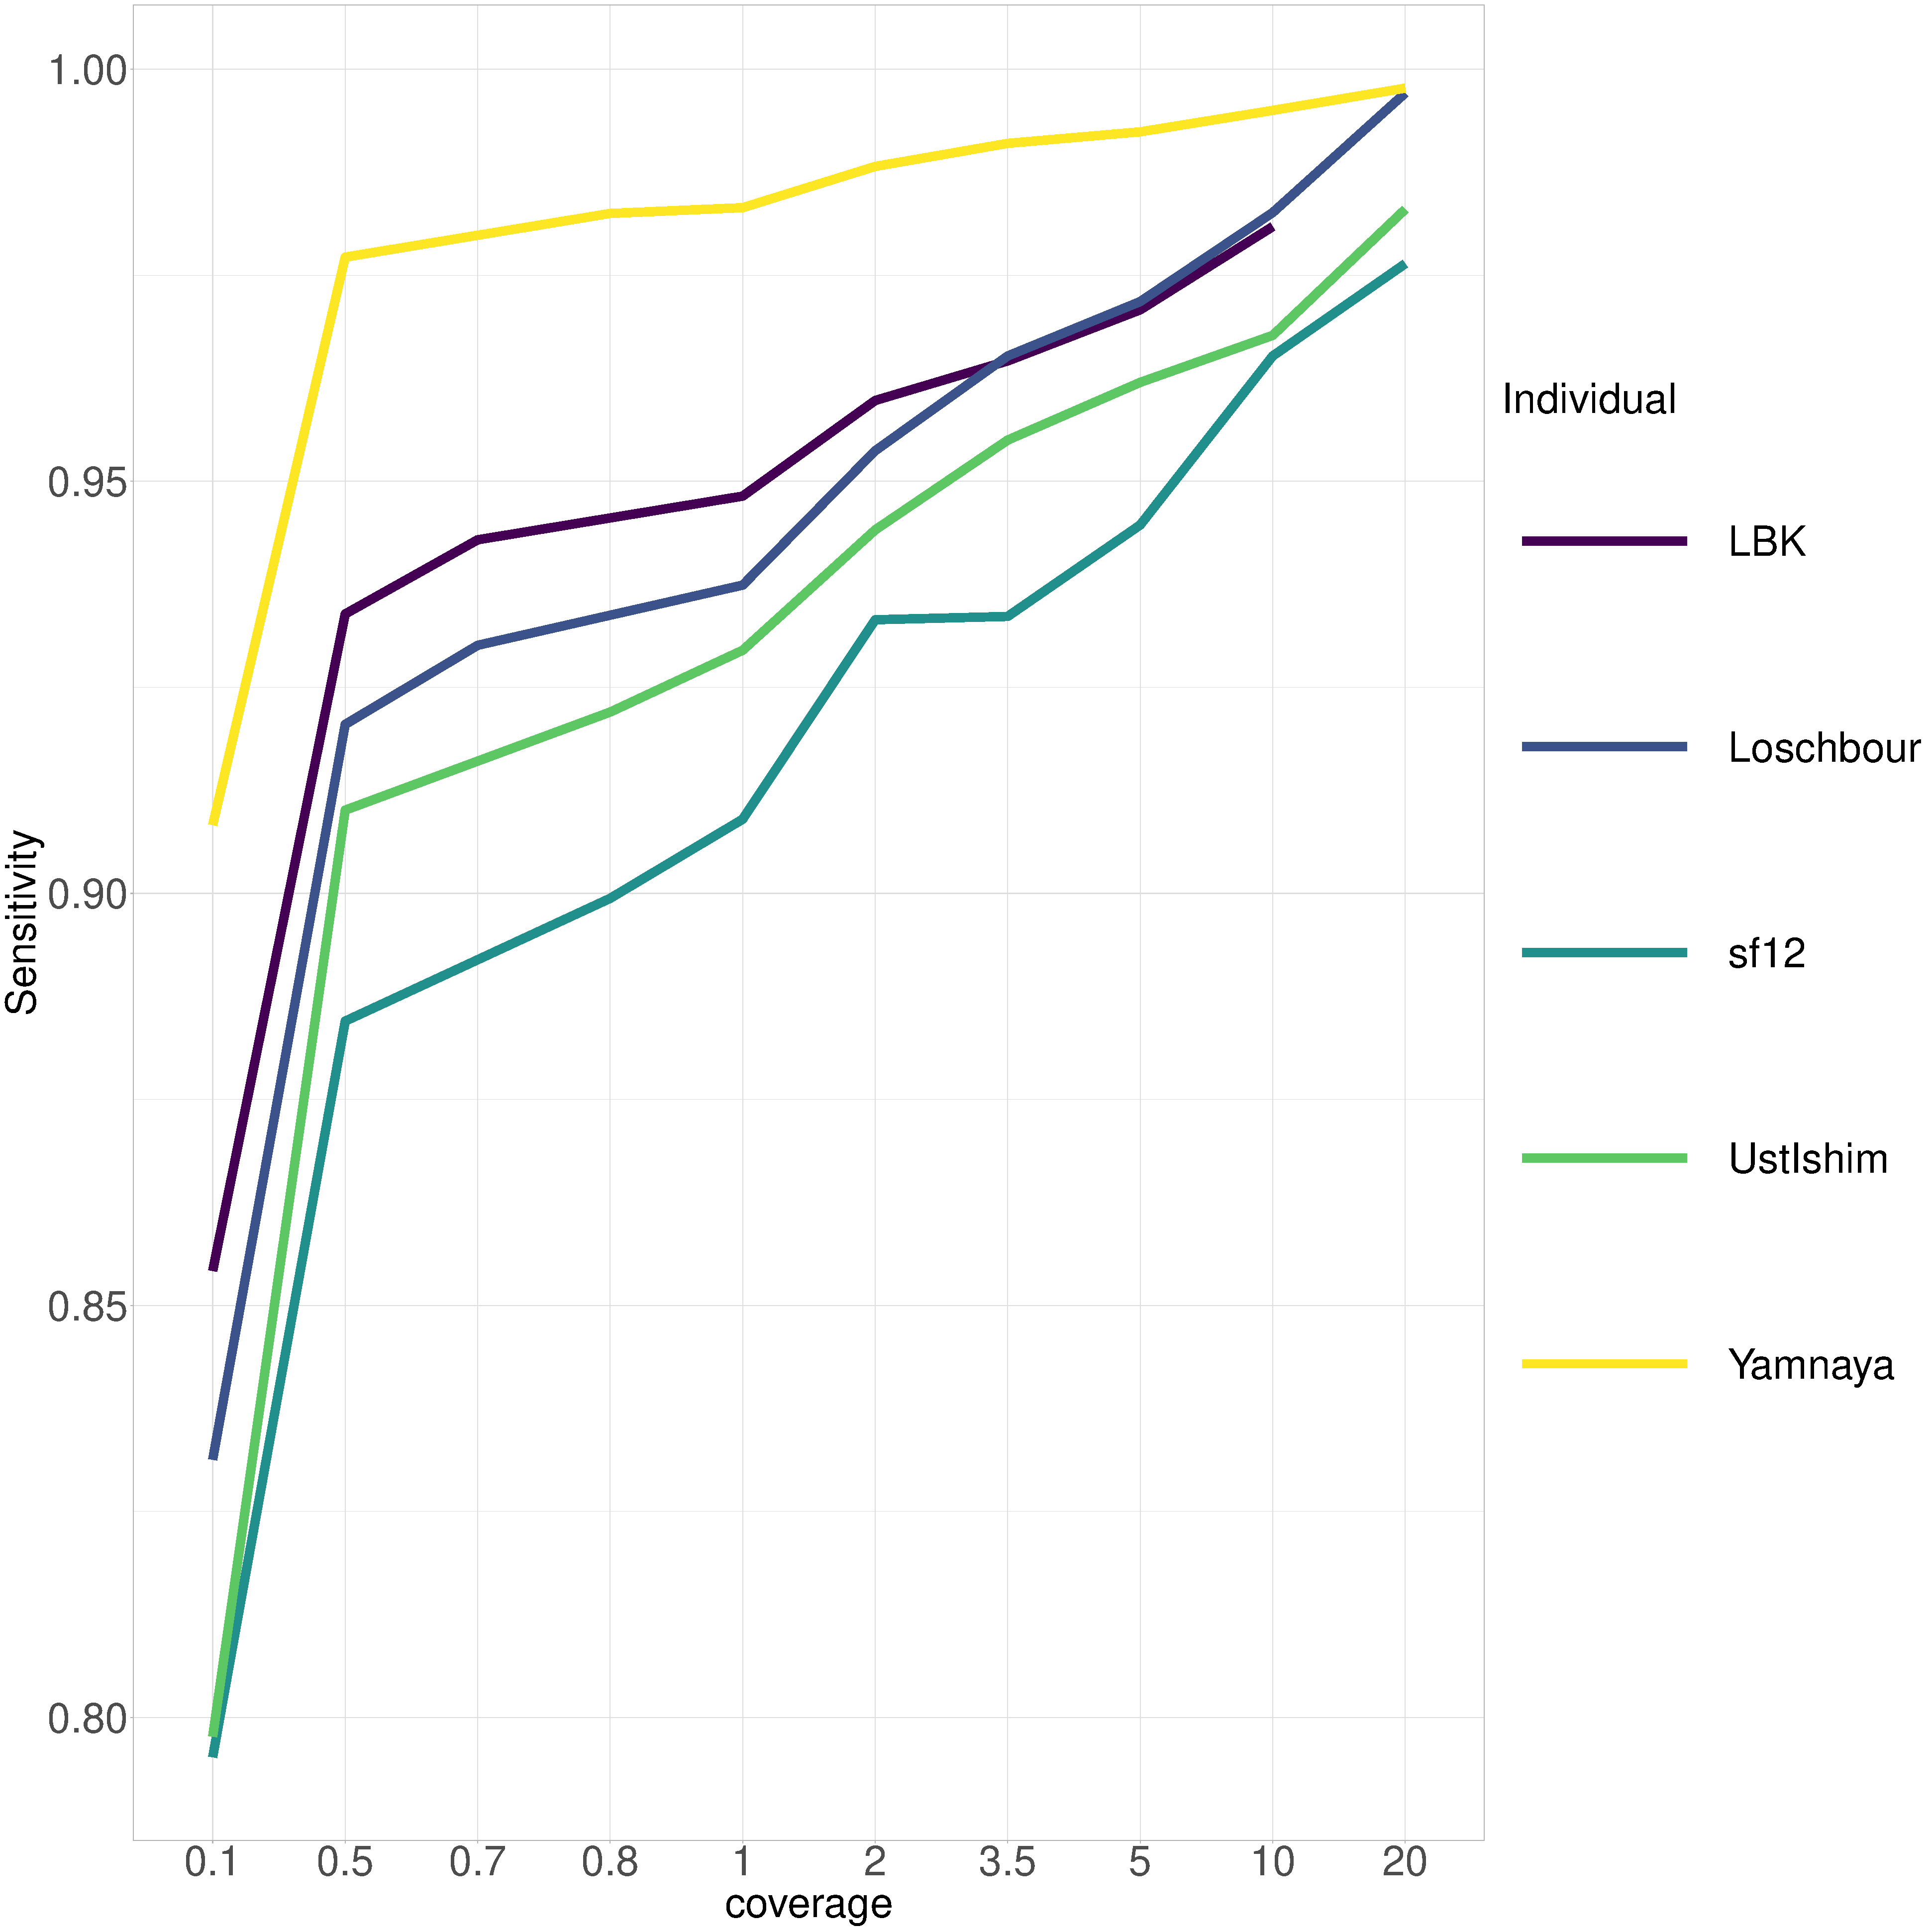
\includegraphics[width=1.0\textwidth]{../images/chapter1/allDownsampled_rtgtools_sensitivity.pdf}
    \caption{Sensitivity of genotype calling at different coverages for different ancient individuals, assuming calls in the full coverage genome are correct,  calculated using rtg-tools.}
    \label{fig:Sensitivity_downsampled_rtgtools}
\end{figure}

\begin{figure}[htp]
    \centering
    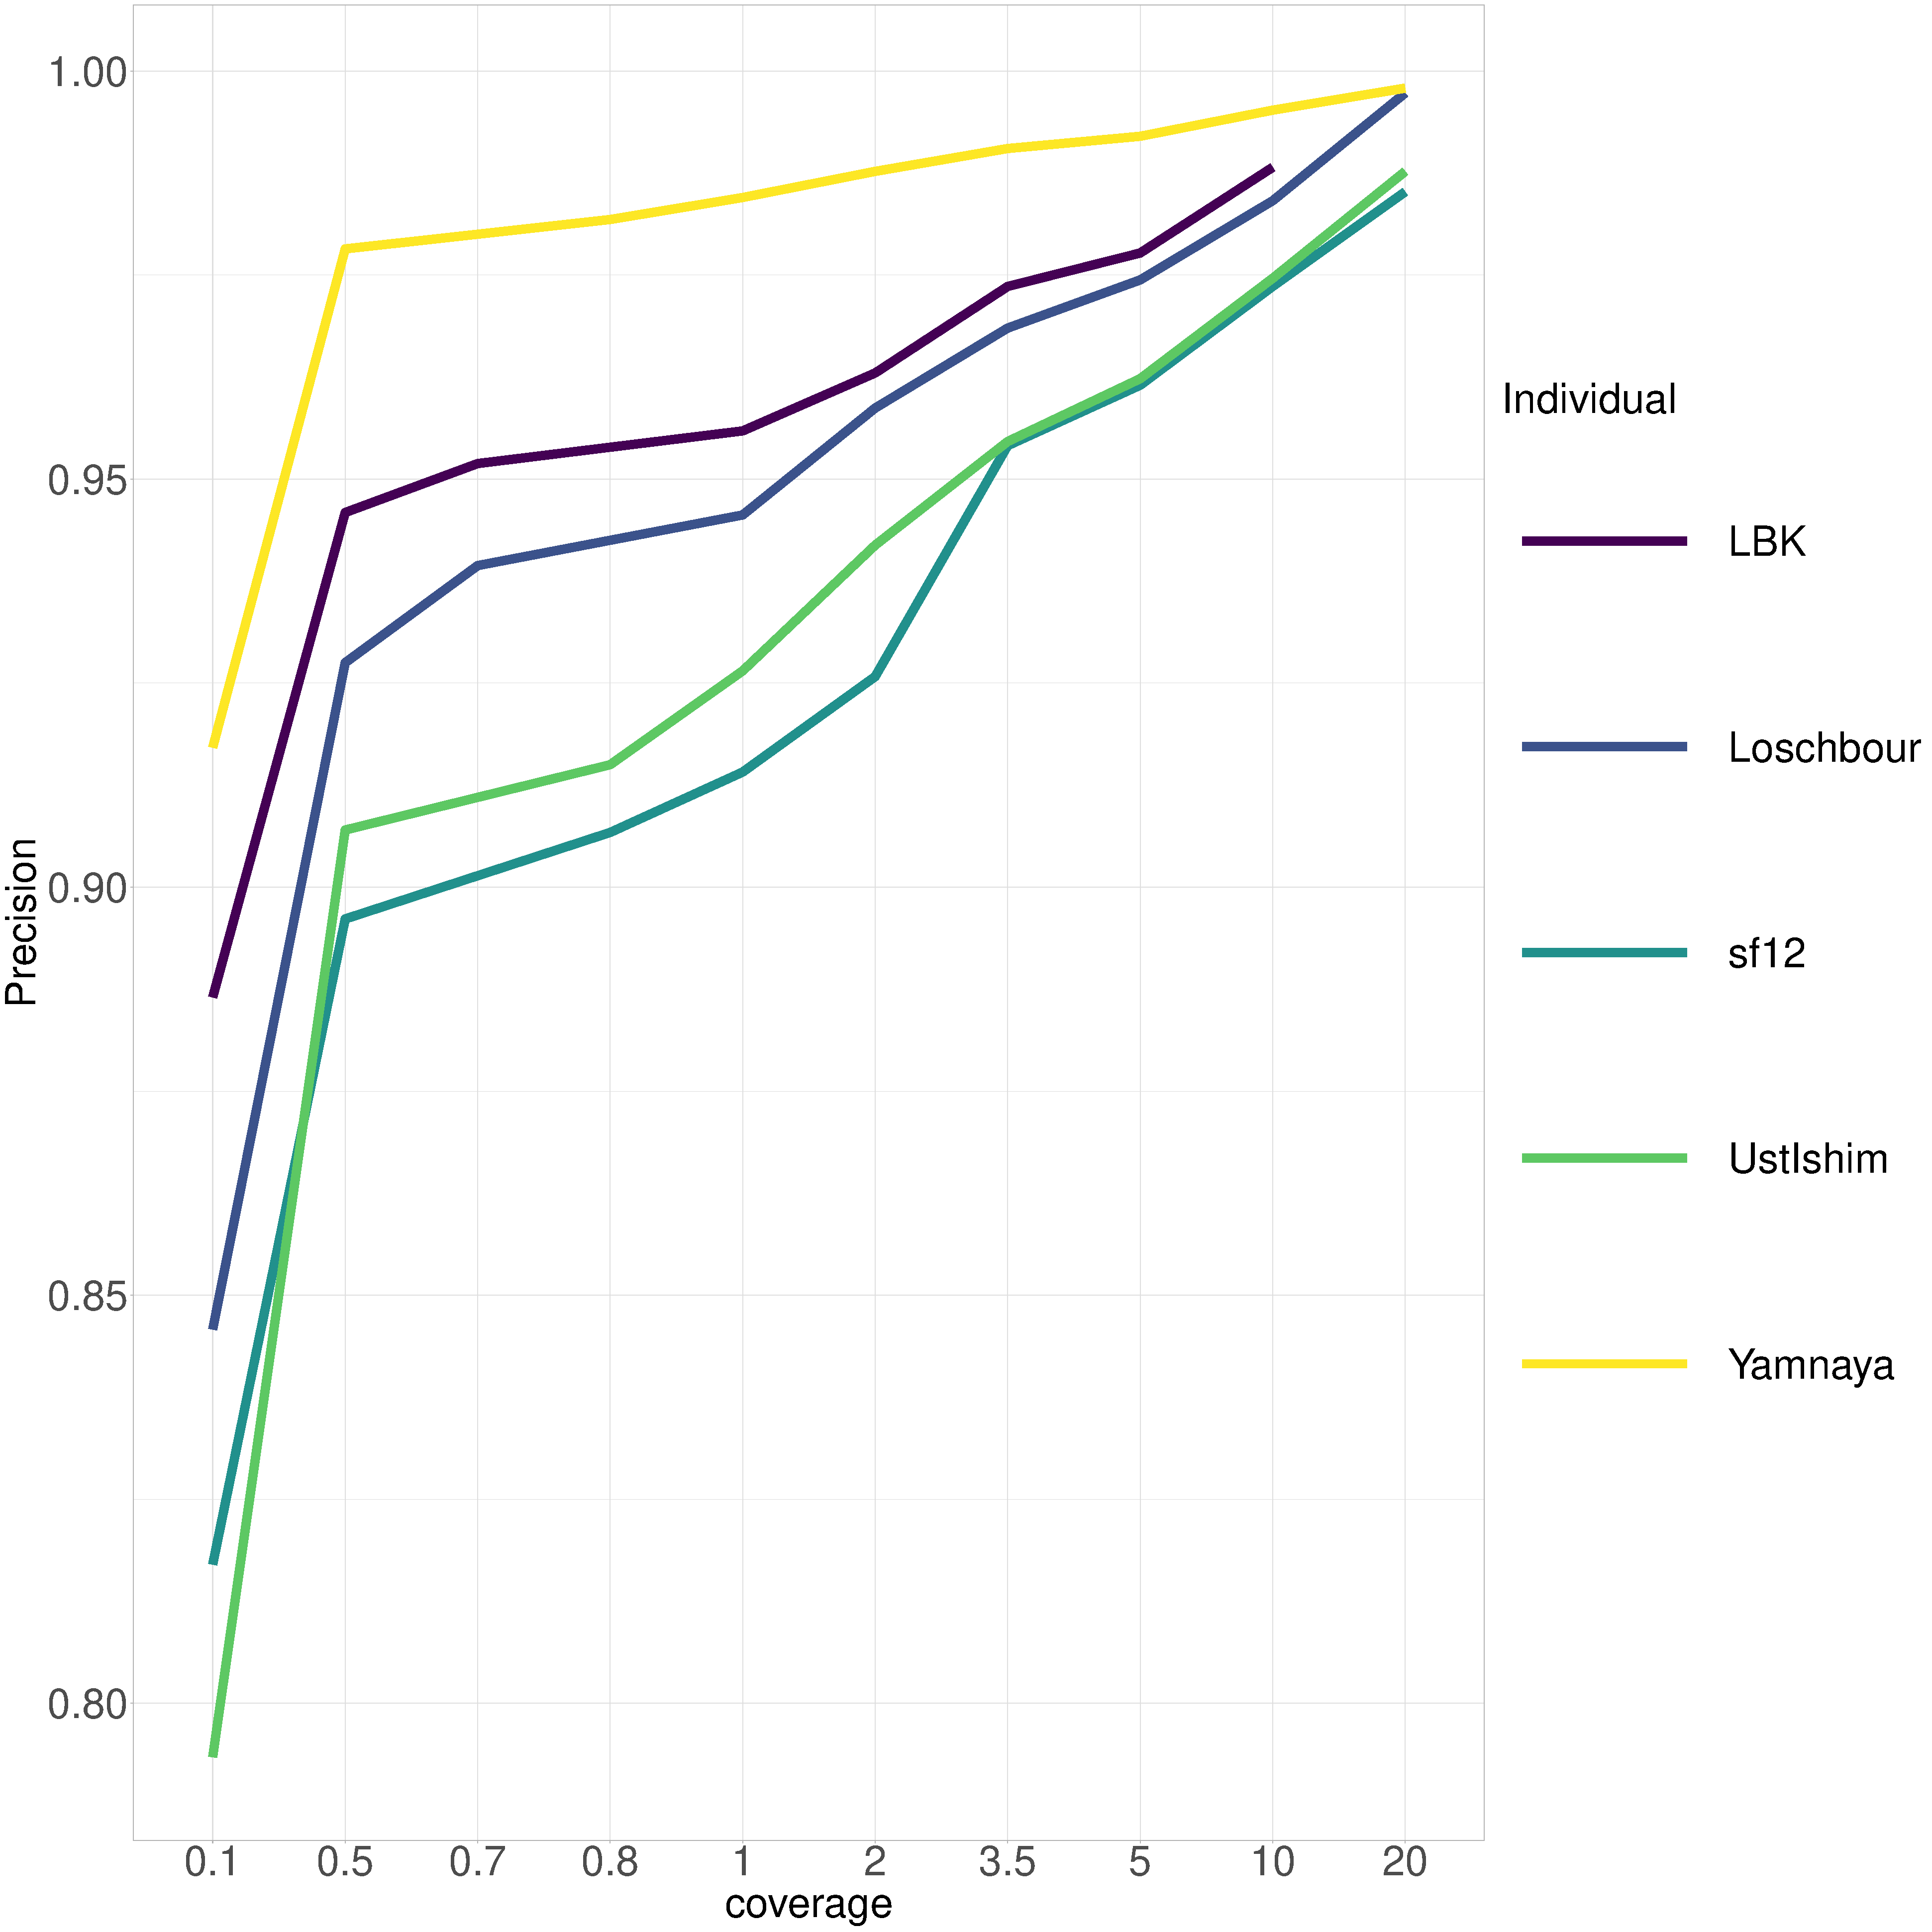
\includegraphics[width=1.0\textwidth]{../images/chapter1/allDownsampled_rtgtools_Precision.pdf}
    \caption{Precision of genotype calling at different coverages for different ancient individuals, assuming calls in the full coverage genome are correct,  calculated using rtg-tools.}
    \label{fig:precision_downsampled_rtgtools}
\end{figure}

As expected, both the overall sensitivity and precision of imputation fell with coverage, with a particularly sharp drop-off in both metrics observed at between 0.5x and 0.1x coverage.

Different downsampled individuals differed in the precision and sensitivity of genotype imputation. At all coverages, Yamnaya had the both the highest sensitivity and precision. This may be because the imputation reference panel contained more individuals who are genetically closer to Yamnaya relative to the other ancient individuals. This is consistent with present-day Europeans containing a high proportion of Yamnaya-like ancestry, relative to e.g. Hunter Gatherer ancestry \cite{Haak2005}. Many studies in present-day individuals have shown that imputation accuracy increases when more haplotypes which are close to the target individual are found in the reference panel \cite{HUANG2009235, delaneau2018integrative}. On the other hand, the sample Ust'Ishim is known to have contributed very little genetic ancestry to present-day populations \cite{Prufer2014} and may therefore have fewer closely matching haplotypes in the reference panel, and a correspondingly lower imputation accuracy. 

Imputation accuracy may also be related to demographic history. Populations which are known to have smaller effective population size, such as Western-Hunter Gathers, also contain longer tracts between individuals which are identical by descent (IBD) and fewer heterozygous positions. As imputation relies on matching IBD tracts between individuals, imputation accuracy increases where individuals share more IBD \cite{kong2008detection}. Additionally, switch-errors during the pre-phasing step of imputation may harm imputation accuracy, so a reduced density of heterozygous positions can improve accuracy. 

\subsection{Phasing accuracy}

I also used rtg-tools to calculate the number of phased heterozygous genotypes where the downsampled individual has the same phasing as the full coverage individual (Fig \ref{fig:phasing_performance_downsampled}). I note that this should not be considered to be the same as estimating the switch error rate, since we do not know that the phasing in the full-coverage individual is the true phase. However, this can be used as a rough proxy for switch errors, since it is known that phasing in lower coverage individuals is likely to be less accurate than those in the high coverage individuals \cite{rubinacci2021efficient}.

\begin{figure}[htp]
    \centering
    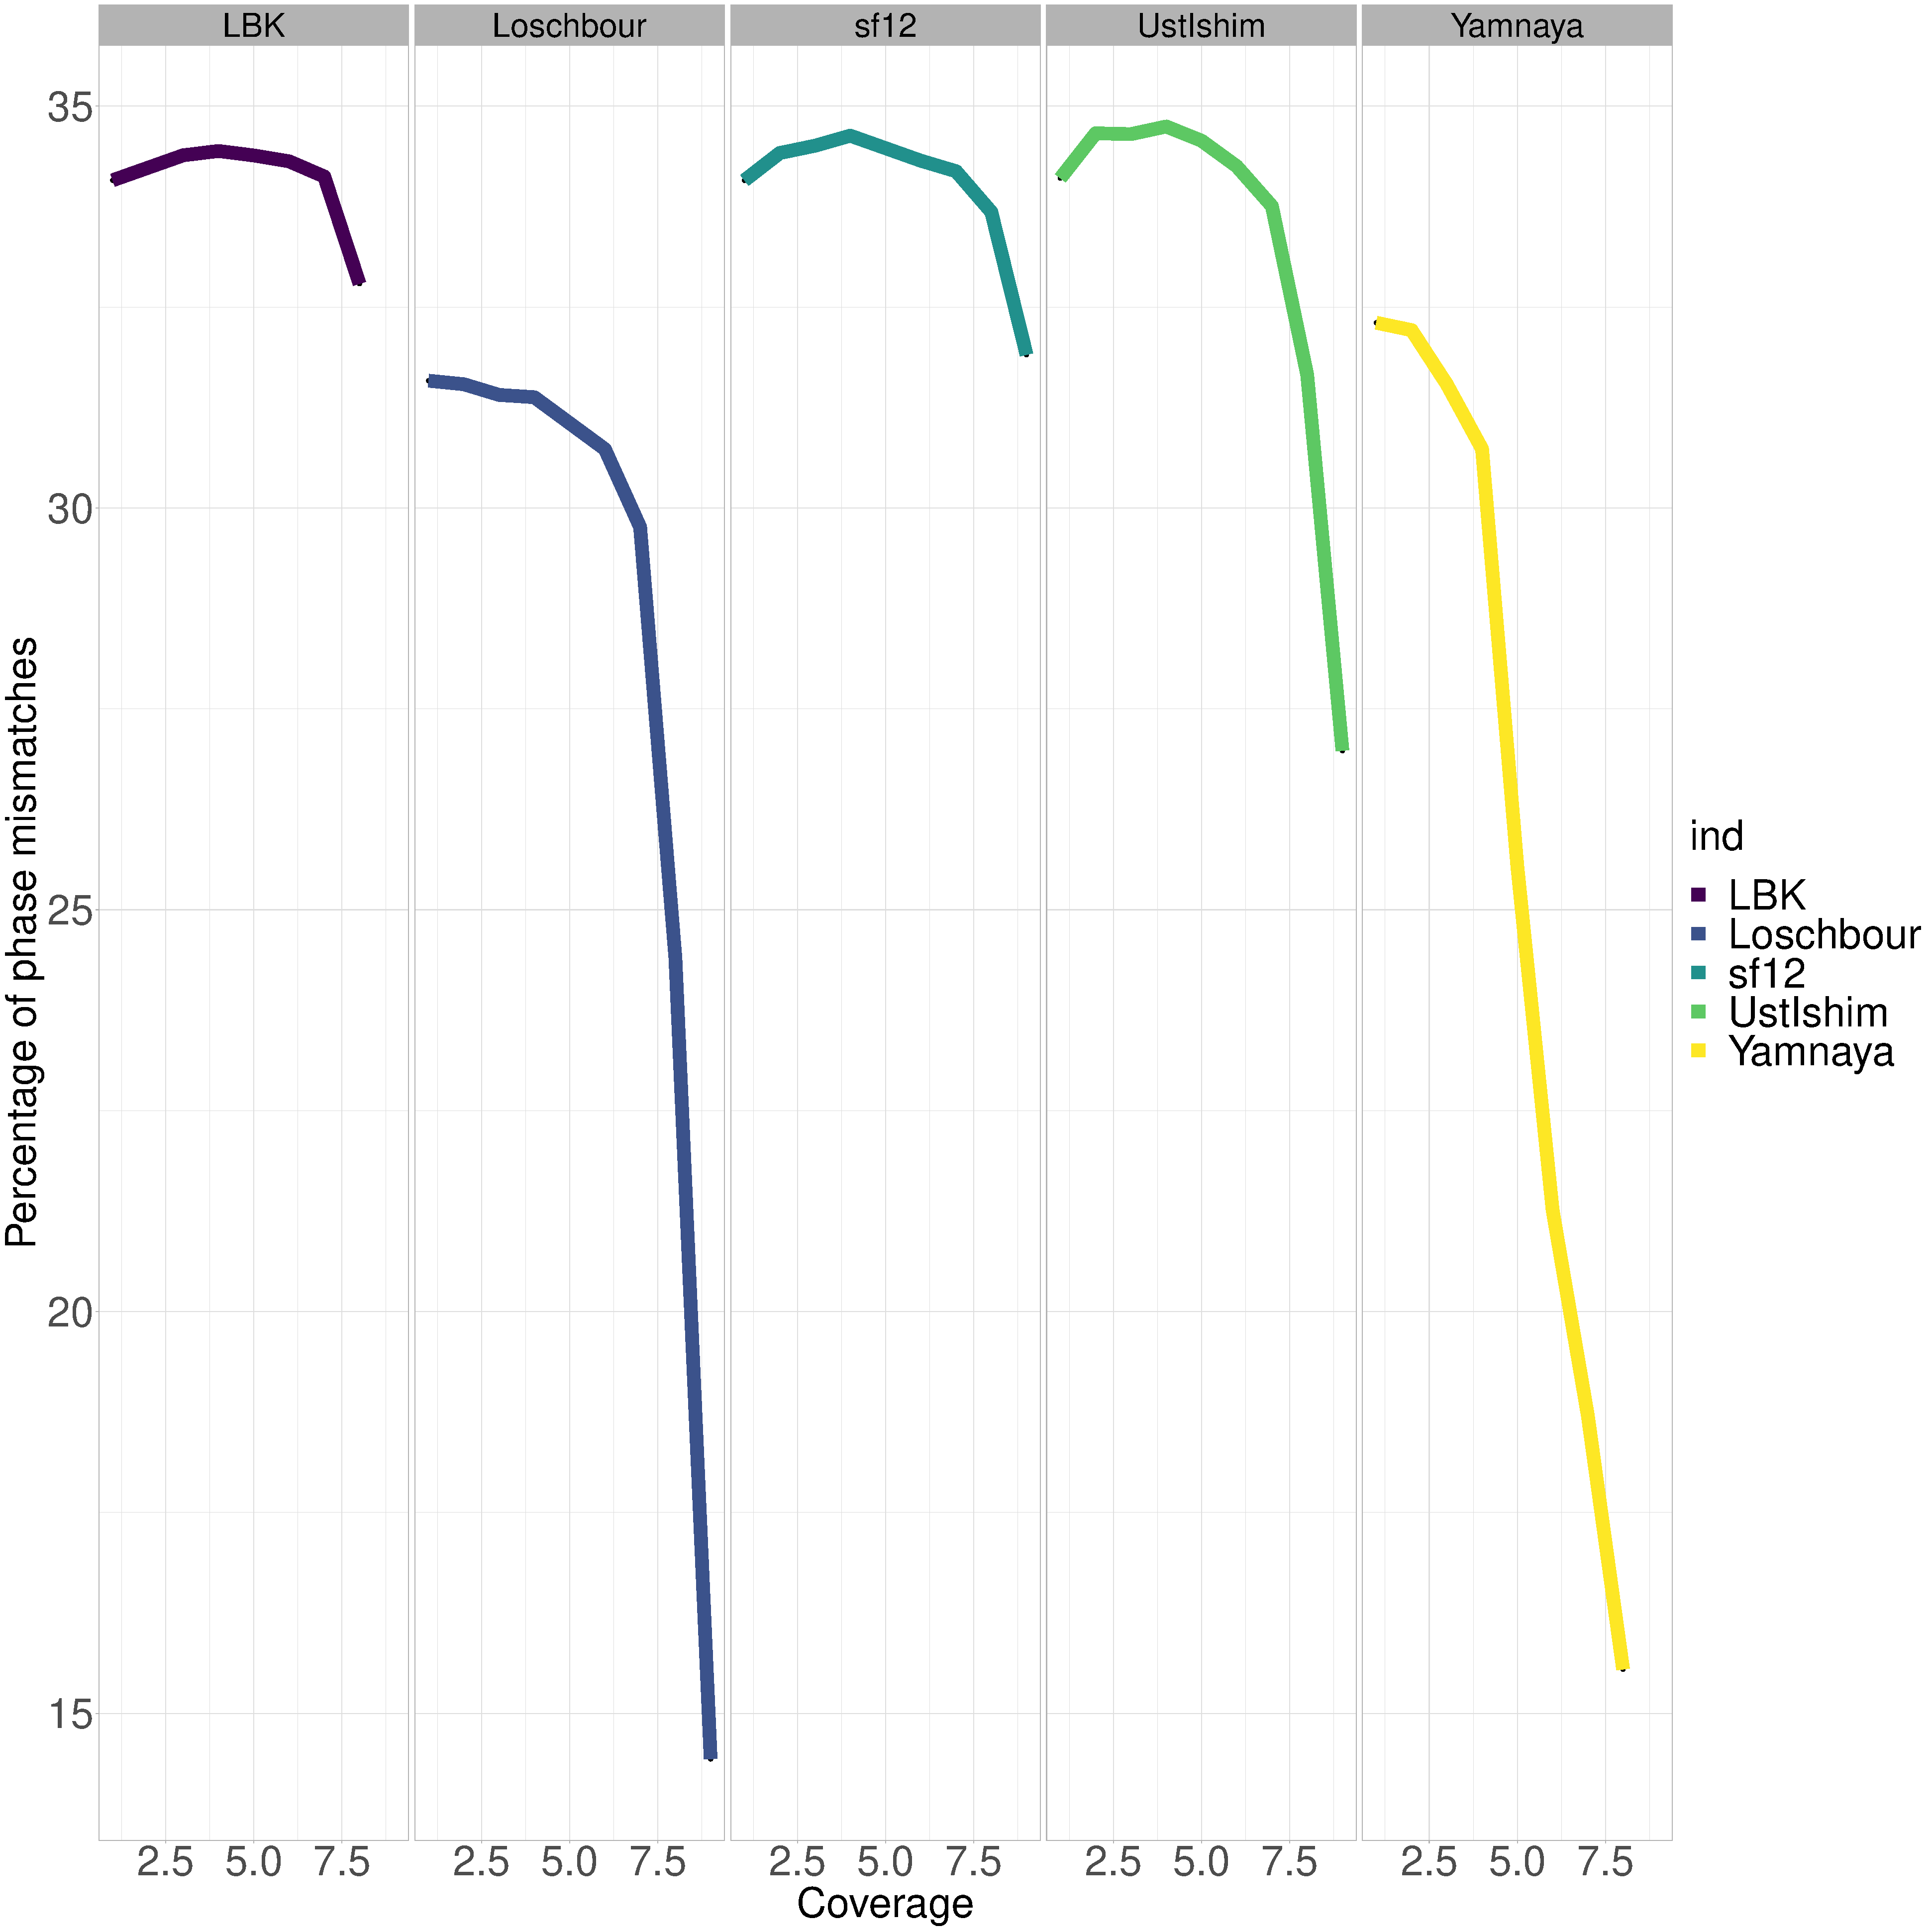
\includegraphics[width=1.0\textwidth]{../images/chapter1/phasing_performance_downsampled.pdf}
    \caption{Percentage of phased genotypes which agree with the reference for each individual and each level of downsampling. Genotypes with phase deemed unresolvable by rtg-tools were excluded from the calculations. Note that these numbers are given as incorrect / (incorrect + correct - unresolved) and so values are in part driven by the relative heterozygosity of each sample.}
    \label{fig:phasing_performance_downsampled}
\end{figure}

\subsection{Validating posterior probability calibration}

When imputing a sample using GLIMPSE, genotype probabilities are emitted. These correspond to the posterior probability that a given genotype within a single individual is correctly called. I assessed how well-calibrated these probabilities are in the Yamnaya 0.1x downsampled individual, using the maximum genotype likelihood at each of the approximately 77 million positions which were processed by GLIMPSE. A high $max(GL)$ for a particular genotype (i.e.\ 0.99) corresponds to a high confidence in the genotype. Alternatively a flat $max(GL)$ (i.e.\ 0.33) corresponds to no information about the genotype. 

I split the genome into 10,000 bins according to $max(GL)$. For each bin, I calculated both the proportion of SNPs which were correctly imputed (i.e. that matched the same high coverage individual) and the mean $max(GL)$ (Fig. \ref{fig:Yamnaya_0.1x_GL_calibration}). If the genotype probabilities are well calibrated, we would expect to see a clear positive linear relationship between $max(GL)$ probability and the probability that genotype matches the full-coverage sample, as we do.

\begin{figure}[htp]
    \centering
    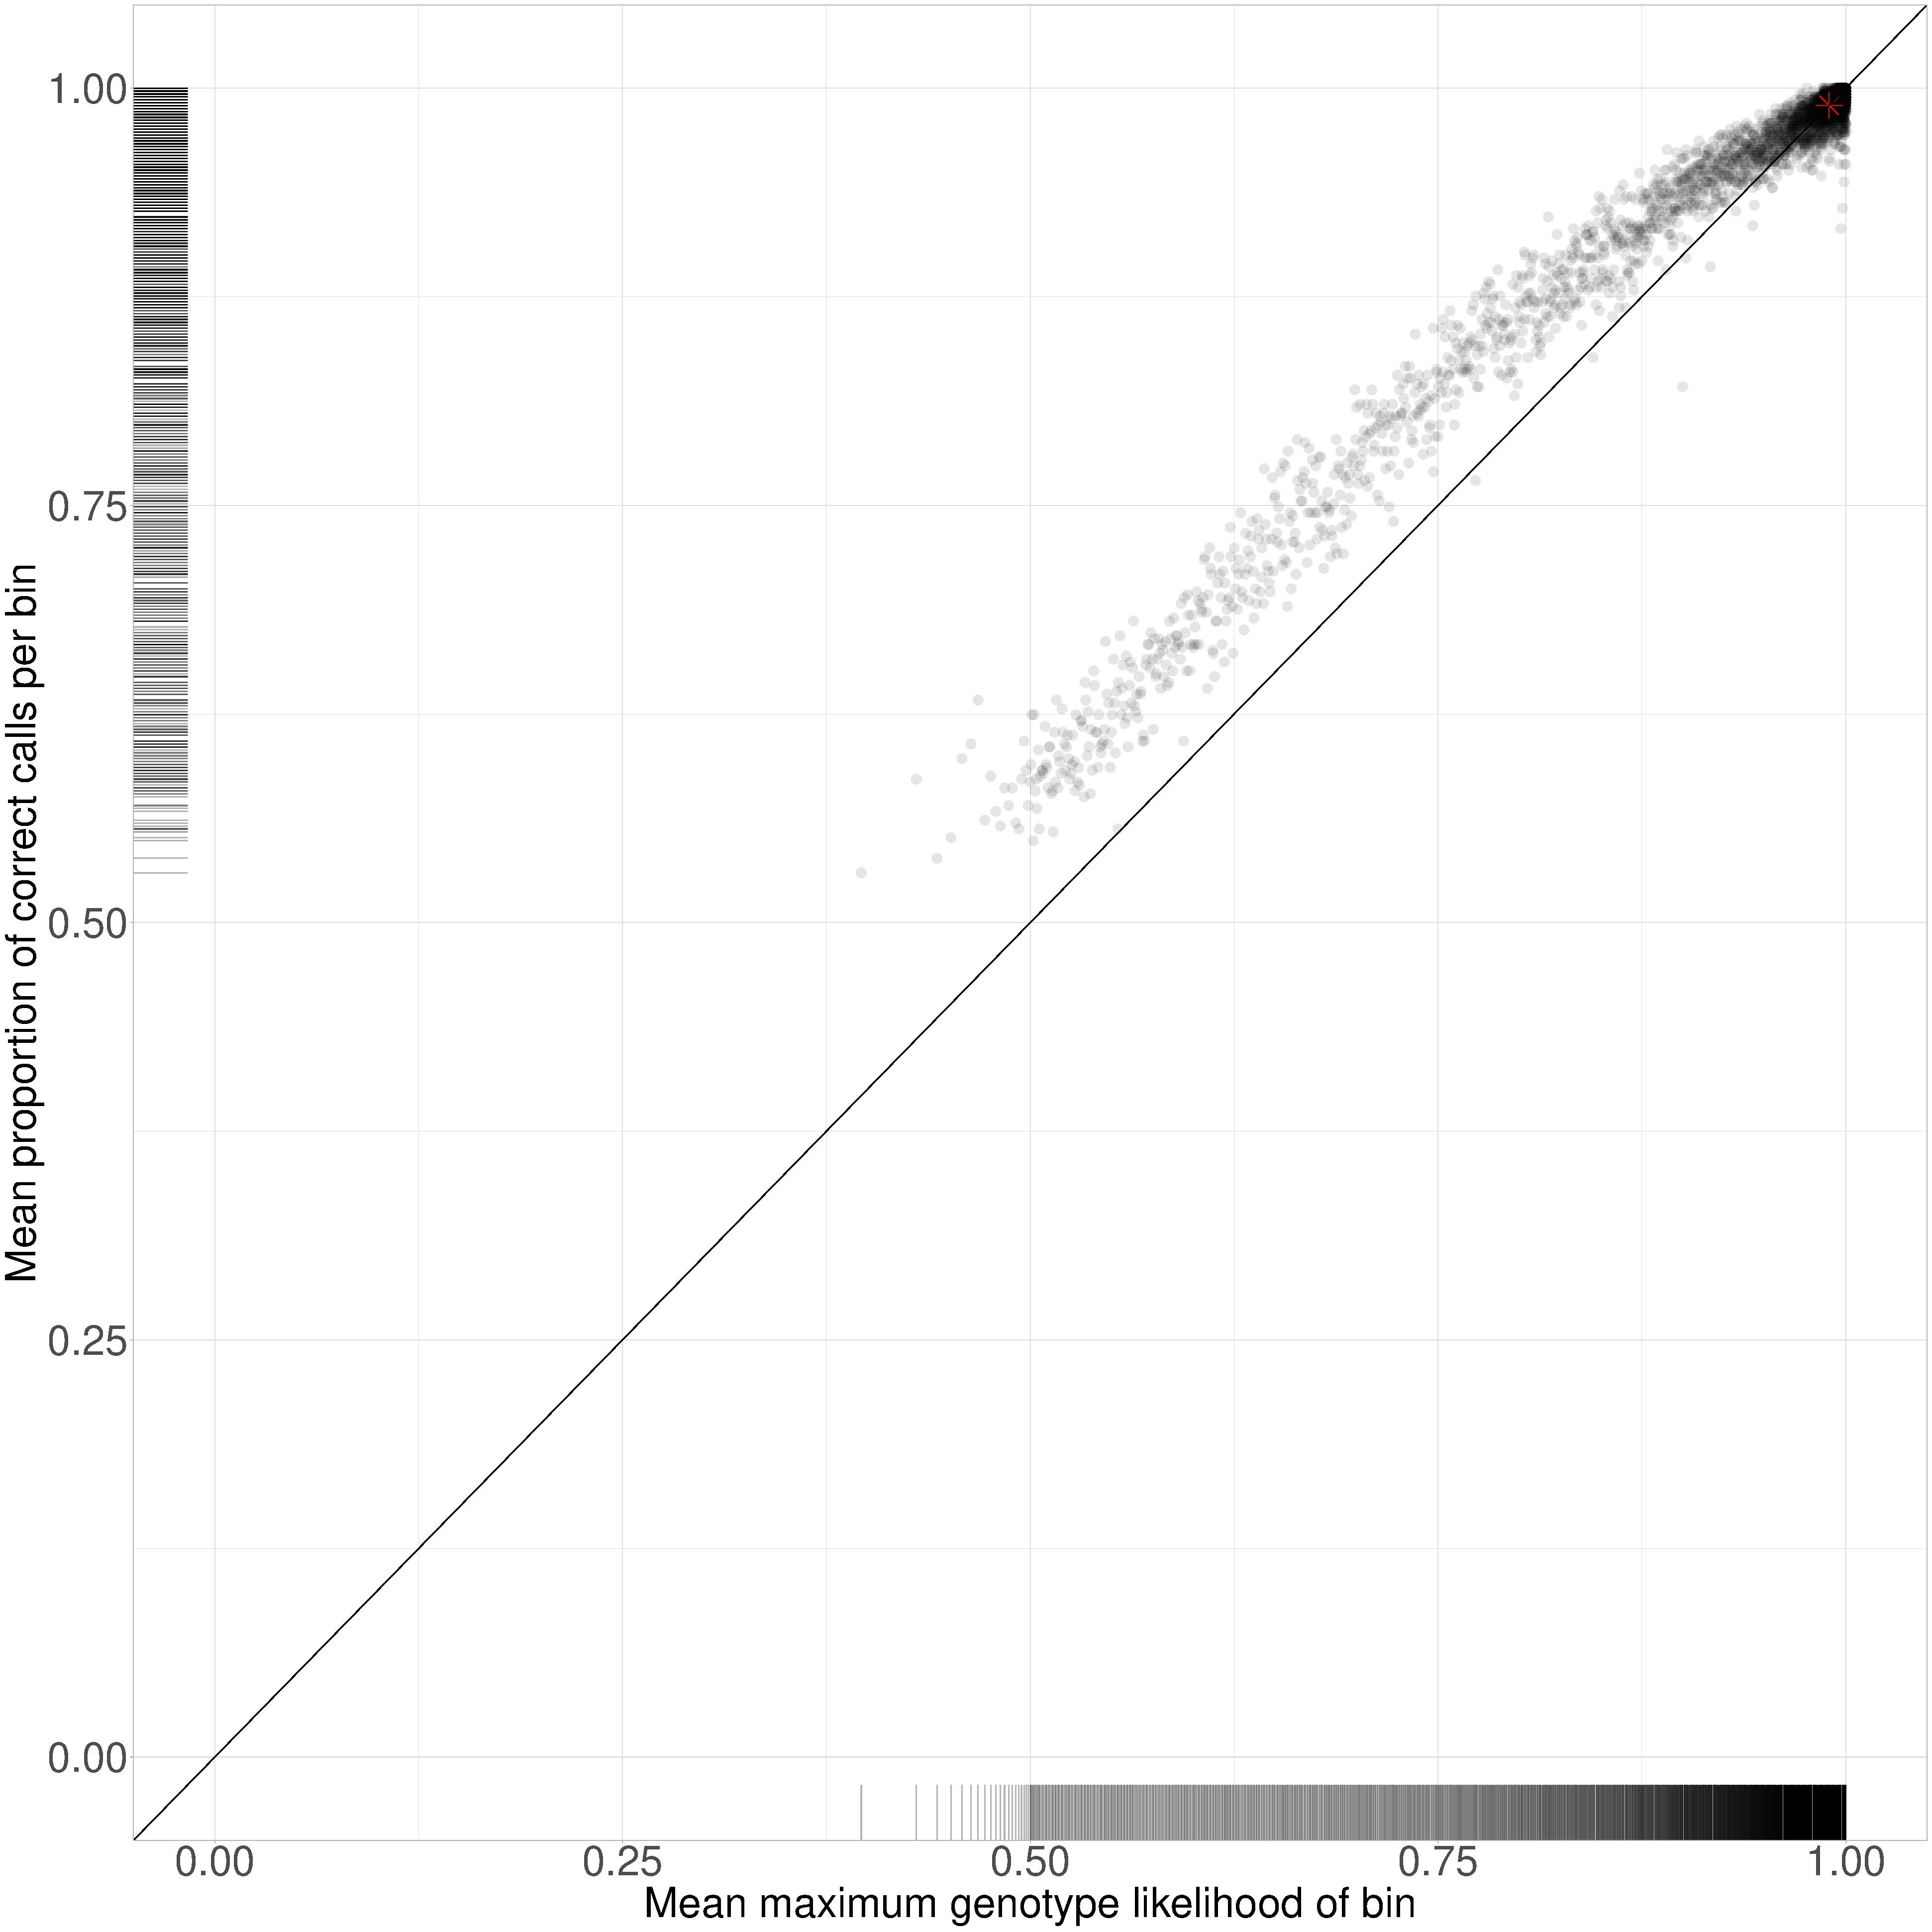
\includegraphics[width=1.0\textwidth]{../images/chapter1/Yamnaya_0.1x_bin.pdf}
    \caption{Relationship between genotype likelihood and probability of genotype call being correct for Yamnaya downsampled to 0.1x coverage. Genome binned by maximum posterior genotype likelihood and mean maximum posterior genotype likelihood (x-axis) and proportion of correct calls per bin (y-axis). Rugs on each margin show the distribution of x and y values. Black line is $y=x$.}
    \label{fig:Yamnaya_0.1x_GL_calibration}
\end{figure}

The probabilities are slightly conservative, in that a majority of the points in Fig. \ref{fig:Yamnaya_0.1x_GL_calibration} are above the $y=x$ line. For example, the mean proportion of correct genotypes within all bins where $0.73 < max(GL) < 0.76$ was 82\%. I performed the same analysis using different samples at different levels of coverage and the results were qualitatively similar (result omitted).

\subsection{ChromoPainter analysis}

To assess the impact of coverage on ChromoPainter analysis, I merged the dataset of downsampled individuals with the `standard set' of ancient reference individuals (124 ancient samples $>2$X coverage) and performed an `all-v-all' painting of the merged dataset, which separately paints each individual as a recipient using all other individuals in the dataset as donors. The `all-v-all' painting was necessary to paint the 124 `standard set' of individuals against one another so that they can act as surrogates in later SOURCEFIND analysis. 

I was interested to see whether a downsampled individual and full coverage had similar copyvectors, or in other words, whether they matched similar amounts to the same donor individuals. To do this, I estimated r-squared between the copyvectors of the full coverage and downsampled individuals.

Fig. \ref{fig:CP_correlation_allSamples_0.1x_0.5x_30x} displays the relationship between copyvectors for each downsampled individual the corresponding full coverage individual for both 0.1x and 0.5x coverage. Each individuals' copyvectors were estimated using the same set of ancient samples as donors.

\begin{figure}[htp]
    \centering
    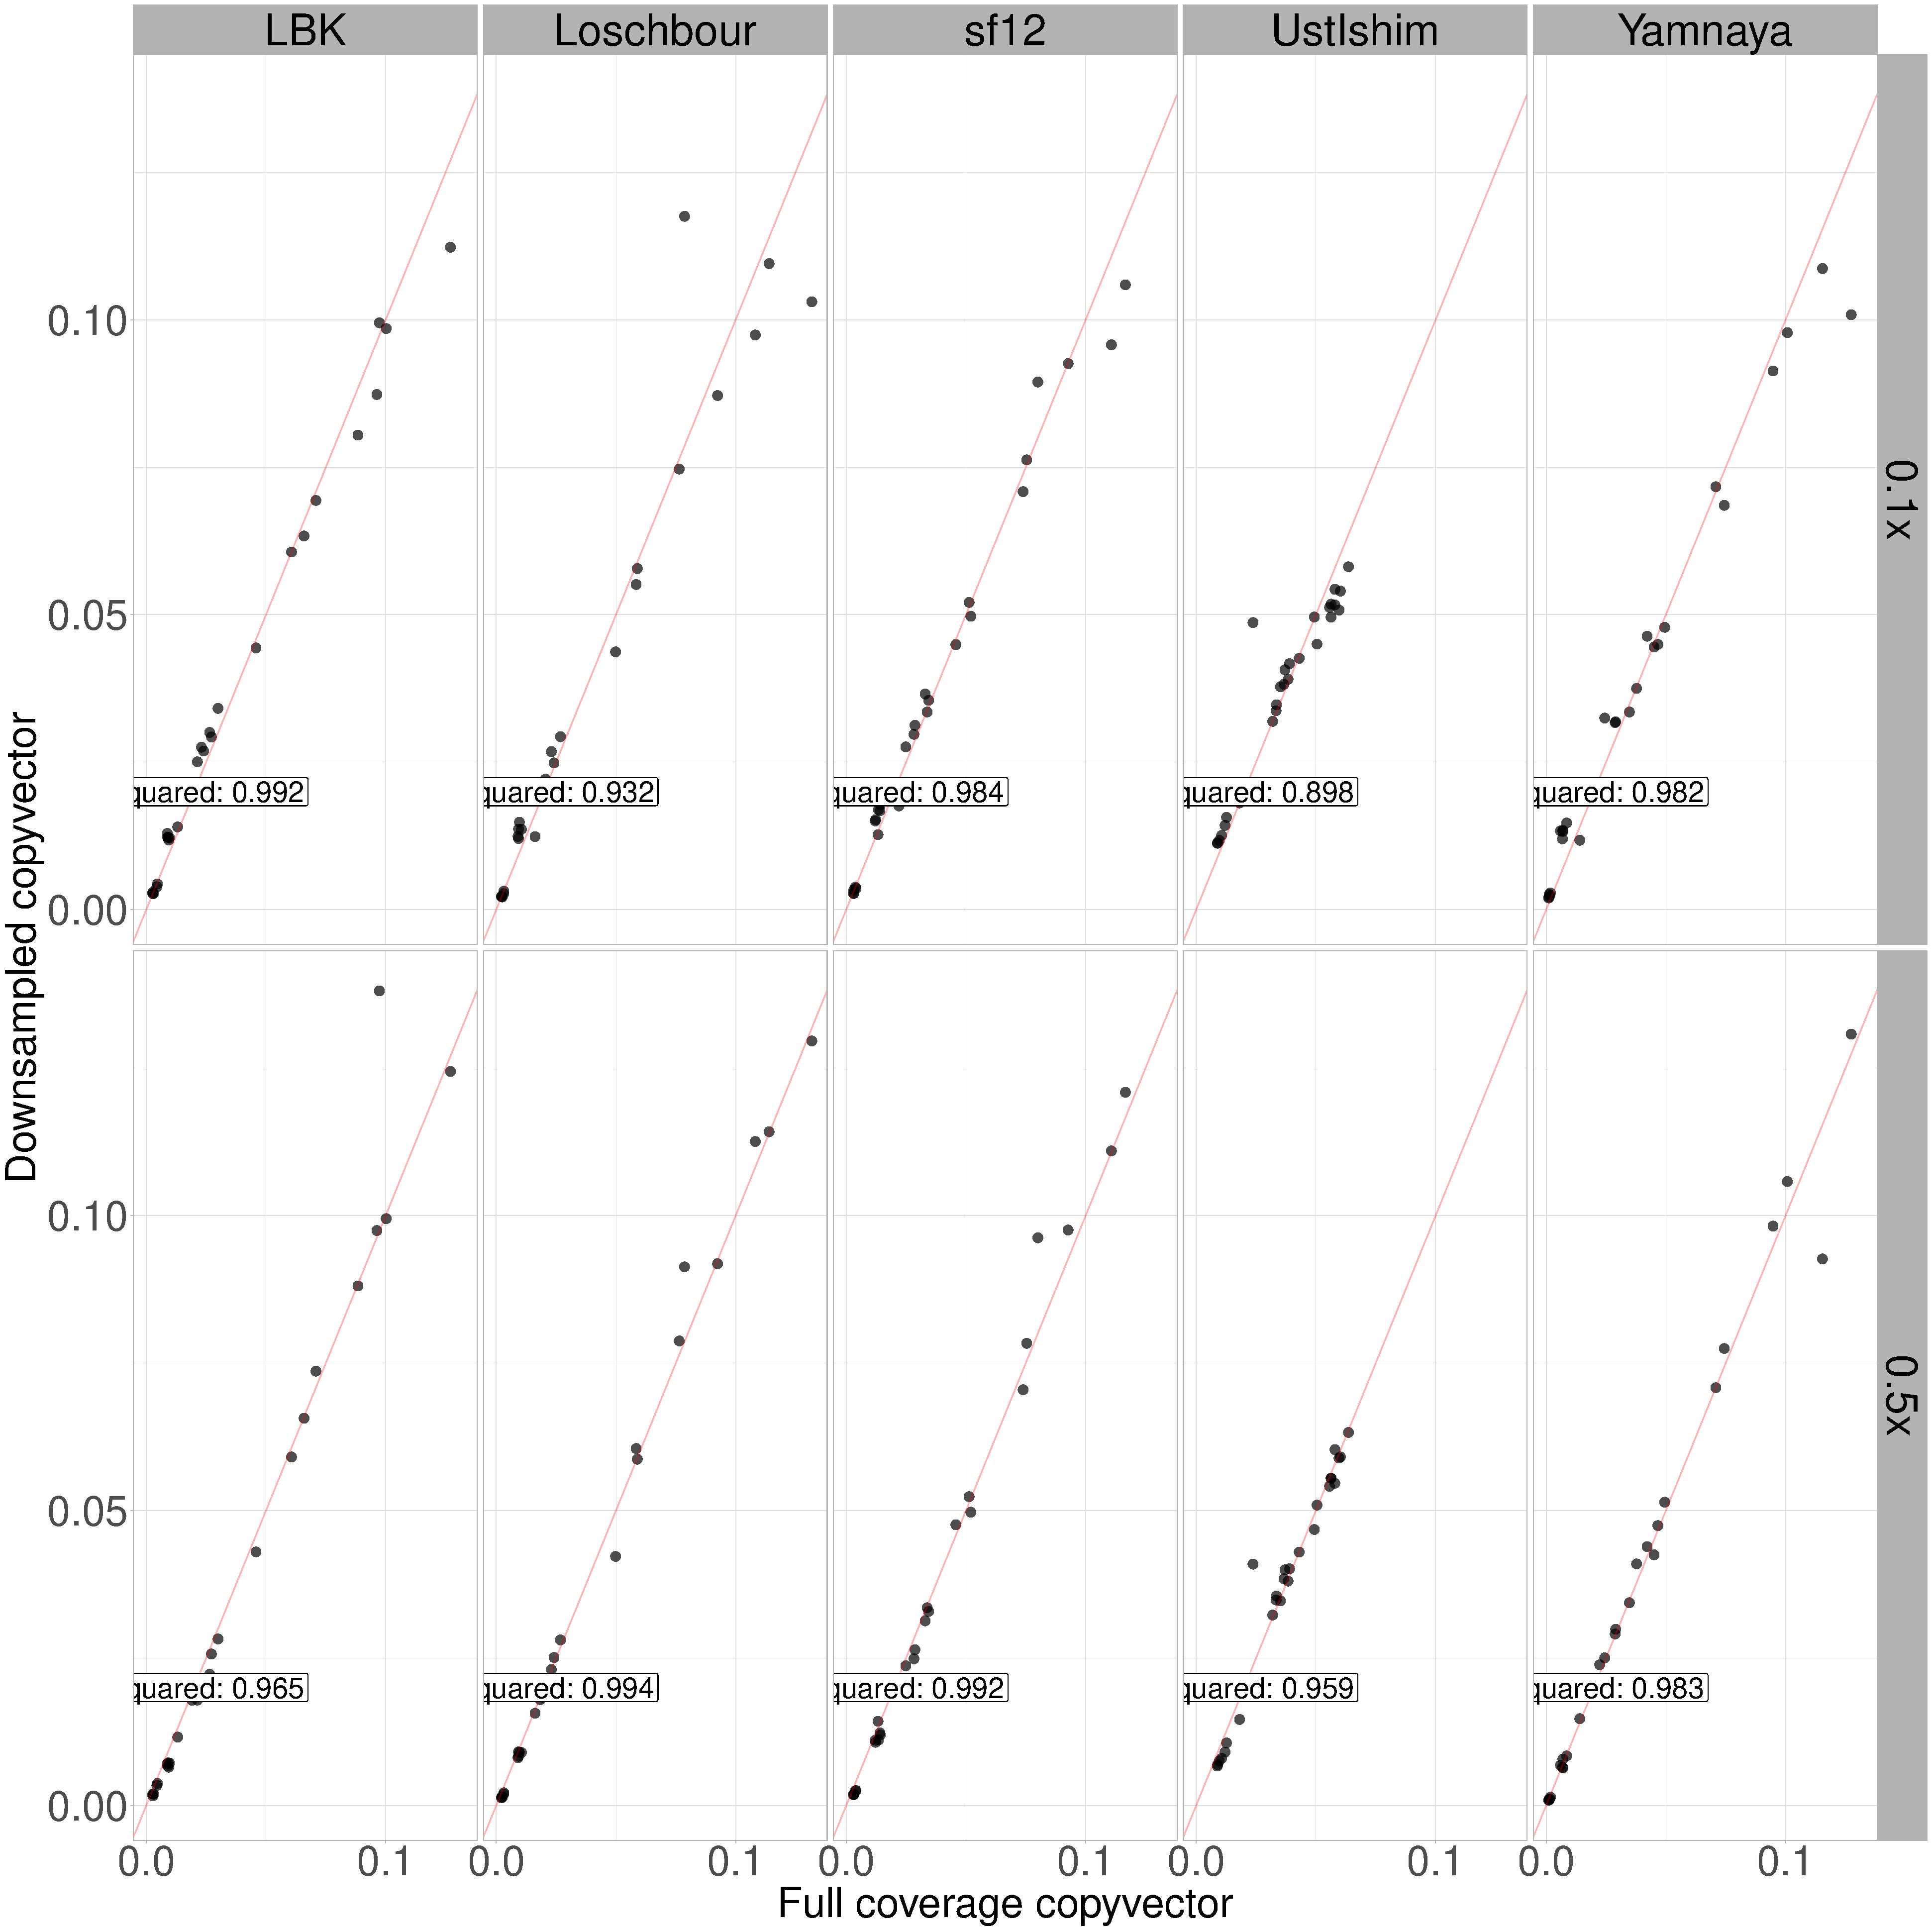
\includegraphics[width=1.0\textwidth]{../images/chapter1/CP_correlation_allSamples_0.1x_0.5x_30x.pdf}
    \caption{For five different samples (columns), the proportion of DNA that each downsampled (y-axis) or full coverage (x-axis) genome matches to each of 125 ancient individuals (dots). Results are shown for 0.1x (top row) and 0.5x (bottom row) downsampled genomes. Points coloured by manual assignment to broad-scale populations. Red line is line of equality ($y=x$).}
    \label{fig:CP_correlation_allSamples_0.1x_0.5x_30x}
\end{figure}

As expected, the TVD between the full-coverage and downsampled copyvectors decreased with coverage. The 0.1x genome had a substantially increased TVD, similar to the much reduced imputation accuracy. For each of the genomes downsampled to 0.1x, a particular difference to the 0.5x downsampled genomes is that the lowest contributing donors contribute more to the 0.1x downsampled genome than to the full coverage genome and that the highest contributing donors contribute less to the 0.1x genome than they do the full coverage genome. Put in other words, the copyvectors at 0.1x are tending towards becoming more `flat', or copying the same amount from each donor individual. 

This can also be seen as `regressing to the prior'. In this case, the prior is copying an equal amount to each donor individual. This can be visualised explicitly by calculating TVD between each downsampled genome and a flat prior, a vector of length $D$, where $D$ is the total number of donor individuals and each element of $D$ is equal to 1 / $D$ (Fig. \ref{fig:TVD_ancients_flat_prior}). This clearly shows the reduced TVD to the flat copyvector for the 0.1x individual relative to other coverages. In later sections, I will discuss whether this is `noise' or `bias' induced by imputation. 

\begin{figure}[htp]
    \centering
    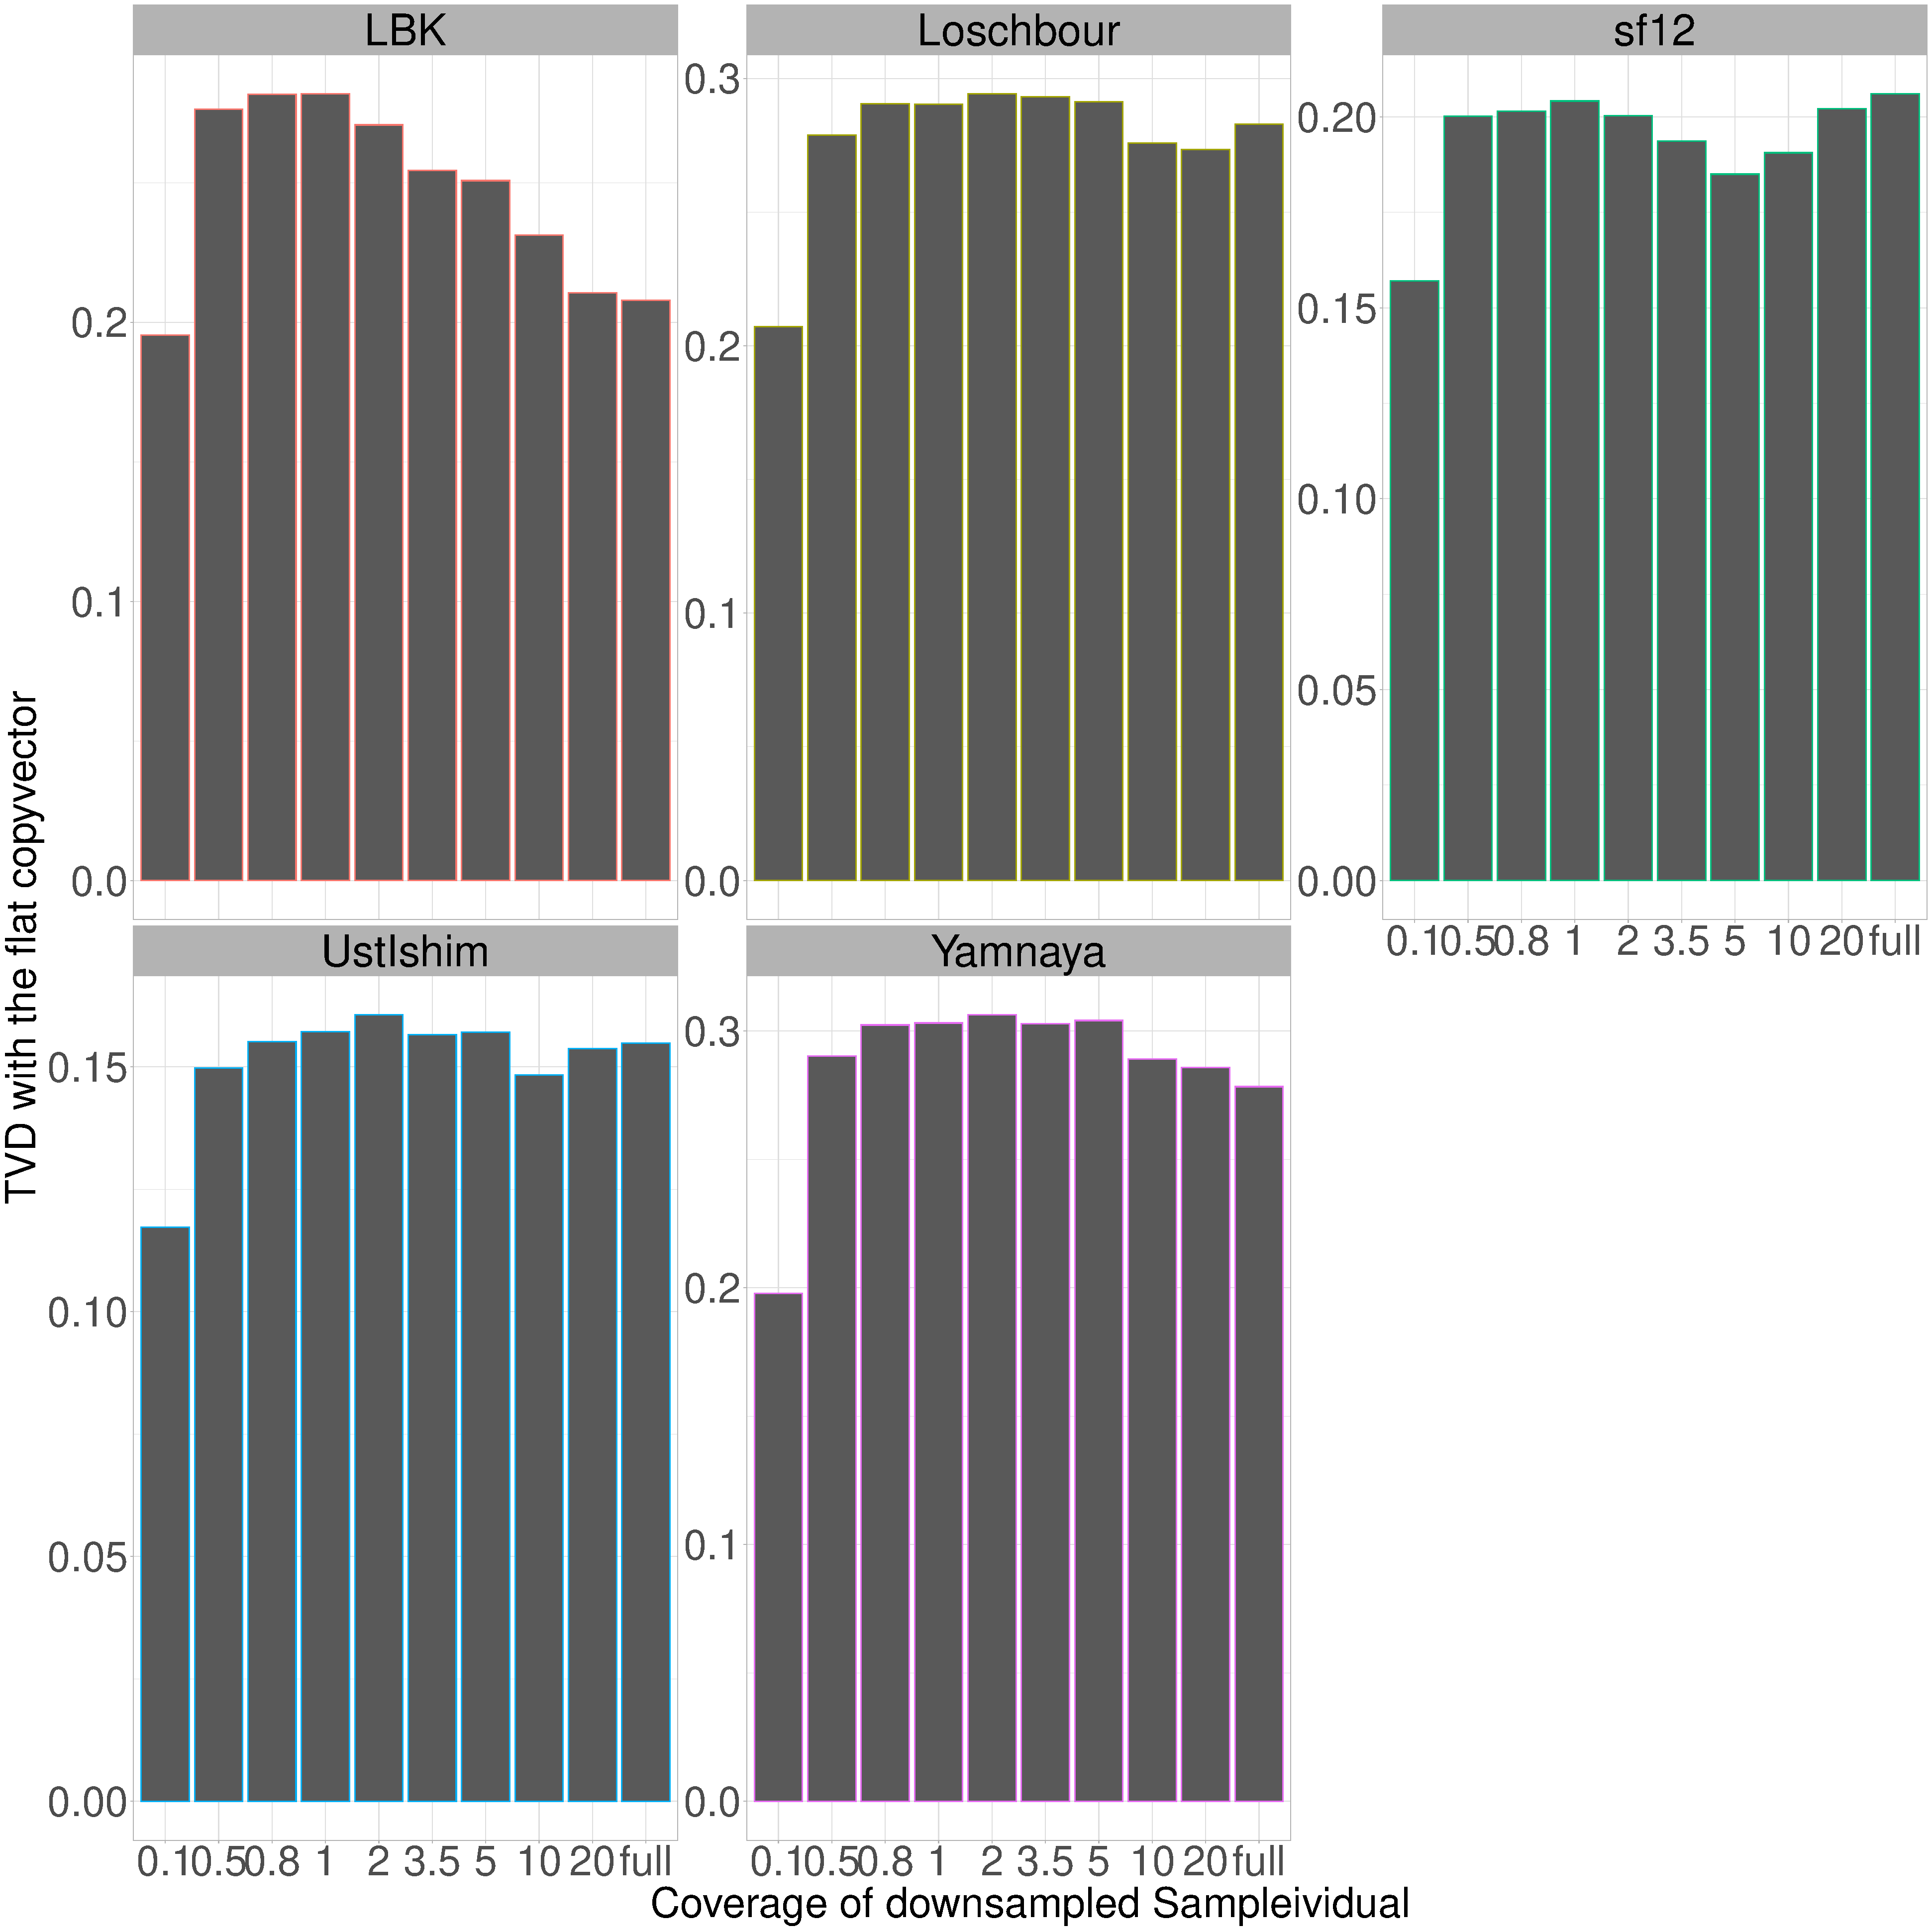
\includegraphics[width=1.0\textwidth]{../images/chapter1/TVD_ancients_flat_prior.pdf}
    \caption{TVD (metric of copyvector dissimilarity between two individuals) between each downsampled ancient individual and a flat copyvector. Flat copyvector equivalent to a vector of length $N$ where each element = $1/N$.}
    \label{fig:TVD_ancients_flat_prior}
\end{figure}

I also considered the effect of coverage on the copyvectors estimated when using modern individuals as donors (Fig. \ref{fig:CP_correlation_allSamples_0.1x_0.5x_30x_moderns}). I merged the downsampled and full coverage ancient individuals with the thousand genomes dataset (described in detail in appendix A.5). As was the case with the all-v-all ancients painting, the TVD between copyvectors was highest for the 0.1x individuals. However, the copyvectors show a strong correlation for 0.5x individuals. 

It should be noted that utility of painting different ancient individuals with a modern reference panel depends on the ancestry and age of the ancient sample. As a comparison, I painted each full coverage and down-sampled ancient against a set donor individuals from 26 present-day populations. The spread of points along the $y=x$ line in Fig. \ref{fig:CP_correlation_allSamples_0.1x_0.5x_30x_moderns} shows how much a particular ancient recipient preferentially copies more from particular modern population over others. LBK, for example, has points which are spread evenly across $y=x$, showing that they copy much more from some populations than others, suggesting modern populations are good for distinguishing this particular ancient sample. On the other hand, the points for Ust'Ishim are clumped together along lower values of $y=x$, showing that the copyvector is relatively flat and that it does not preferentially copy from some populations to the same degree that LBK does. This is consistent with findings that UstIshim did not contribute ancestry towards present-day populations \cite{Fu2014}. Accordingly, relatively less useful information is obtained from painting Ust'Ishim with a modern reference panel than LBK.

\begin{figure}[htp]
    \centering
    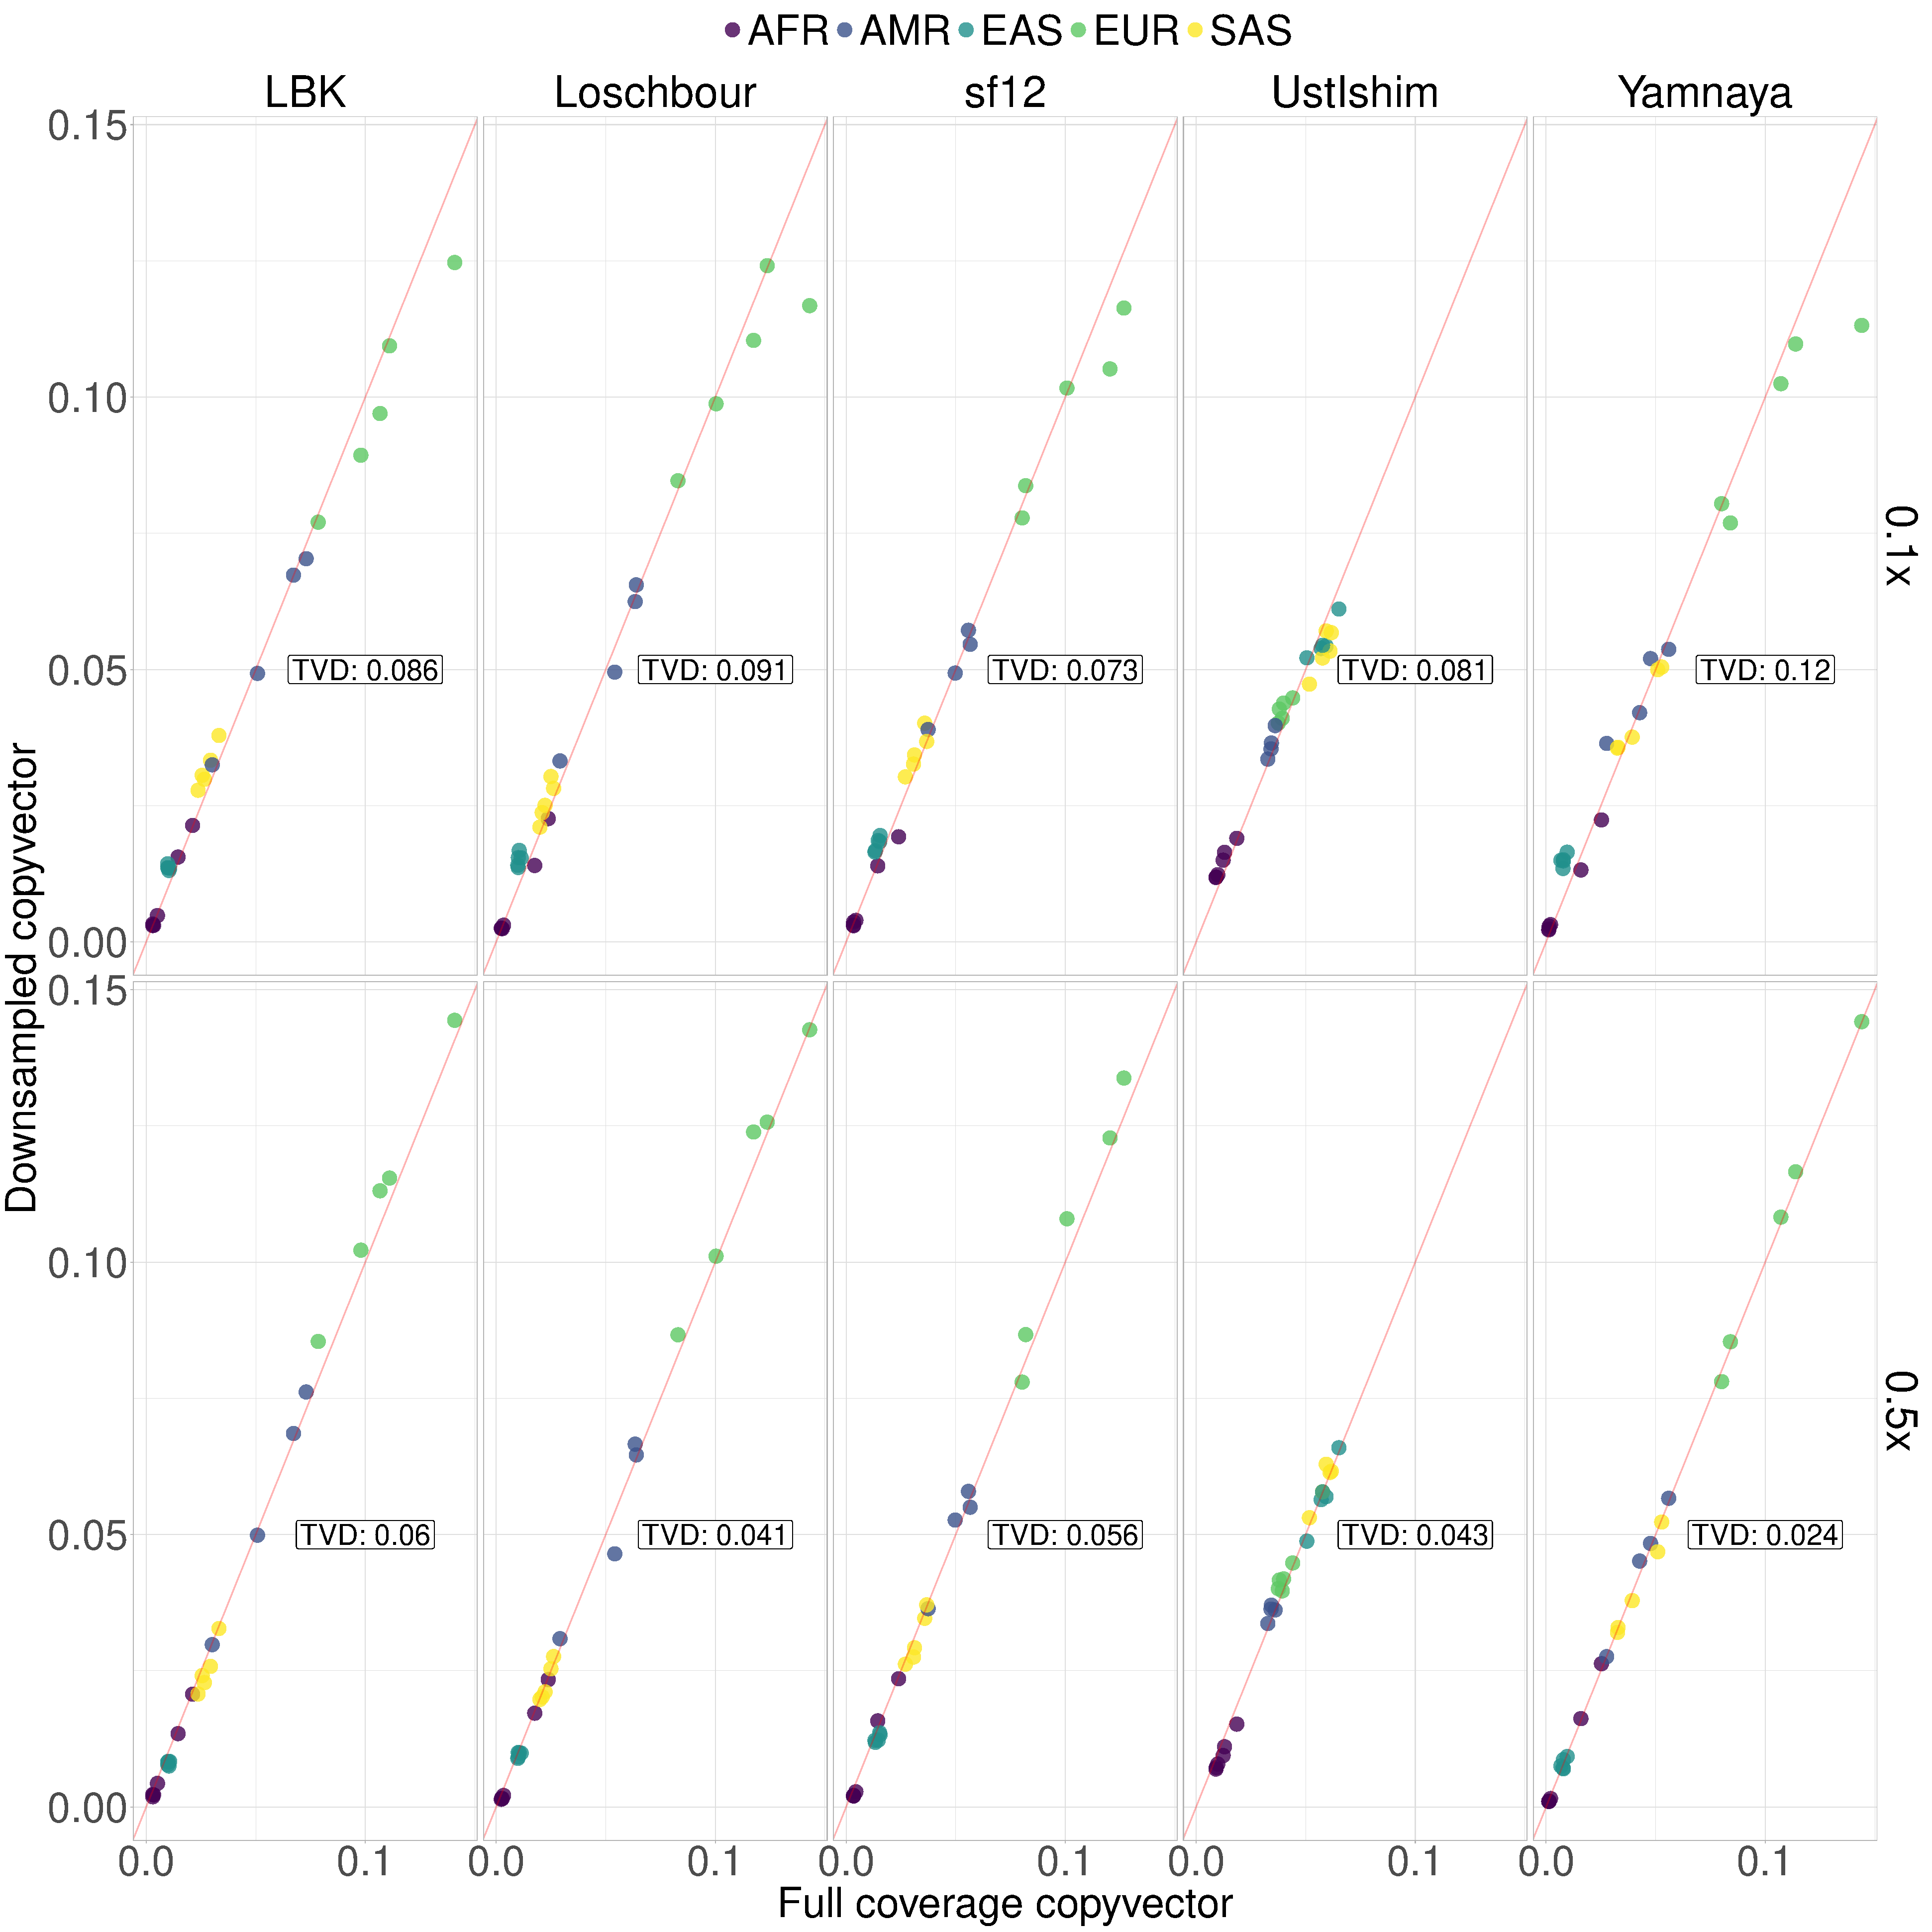
\includegraphics[width=1.0\textwidth]{../images/chapter1/CP_correlation_allSamples_0.1x_0.5x_30x_moderns.pdf}
    \caption{For five different samples (columns), the proportion of DNA that each downsampled (y-axis) or full coverage (x-axis) genome matches to individuals from each of 26 present-day populations (dots). Red line is $y=x$.}
    \label{fig:CP_correlation_allSamples_0.1x_0.5x_30x_moderns}
\end{figure}

Principle component analysis (PCA) is a widely used technique to visualise the relative genetic diversity of different individuals. PCA can be performed on the chunklengths matrix in a similar way to a PCA on the genotype dosage matrix, which is often employed in ancient DNA studies. Visualising whether downsampled individuals cluster close to the same sample at full-coverage is a useful way of determining whether the copyvectors of the downsampled individual reflect those of the full-coverage individual.

To avoid the confounding effect of having two almost identical individuals on a PCA (e.g.\ the 1x and 0.5x downsamples of the same individual), I performed PCA separately for each ancient individual (see methods section x for full details) (Fig. \ref{fig:PCA_panel_allInds_allCoverage}). 

The position of the full coverage individuals are consistent with prior knowledge about their ancestry. For example, Loschbour is positioned alongside other Hunter Gatherers, who are highly differentiated from the later Neolithic farmers and Bronze Age Europeans. sf12 clusters with the other Scandinavian Hunter Gatherers in the dataset. Yamnaya is differentiated from the group of Bronze Age individuals and situated close to individuals from the Poltavka and Srubnaya culture. LBK is located with other individuals from the early to middle Neolithic in central Europe. Consistent with sharing little ancestry with any group over another, UstIshim is positioned close to the central Bronze Age mass, where most of the individuals in the PCA are located. 

For all levels of downsampling other than the 0.1x, the downsampled and full coverage genomes were positioned very closely to one another on the PCA. When considering all downsampled individuals, a pattern emerges whereby the genome downsampled to 0.1x for each individual is `pulled' towards the origin of the PCA. This may reflect a `homogenisation' of low coverage genomes when many genotypes are imputed.

\begin{figure}[htp]
    \centering
    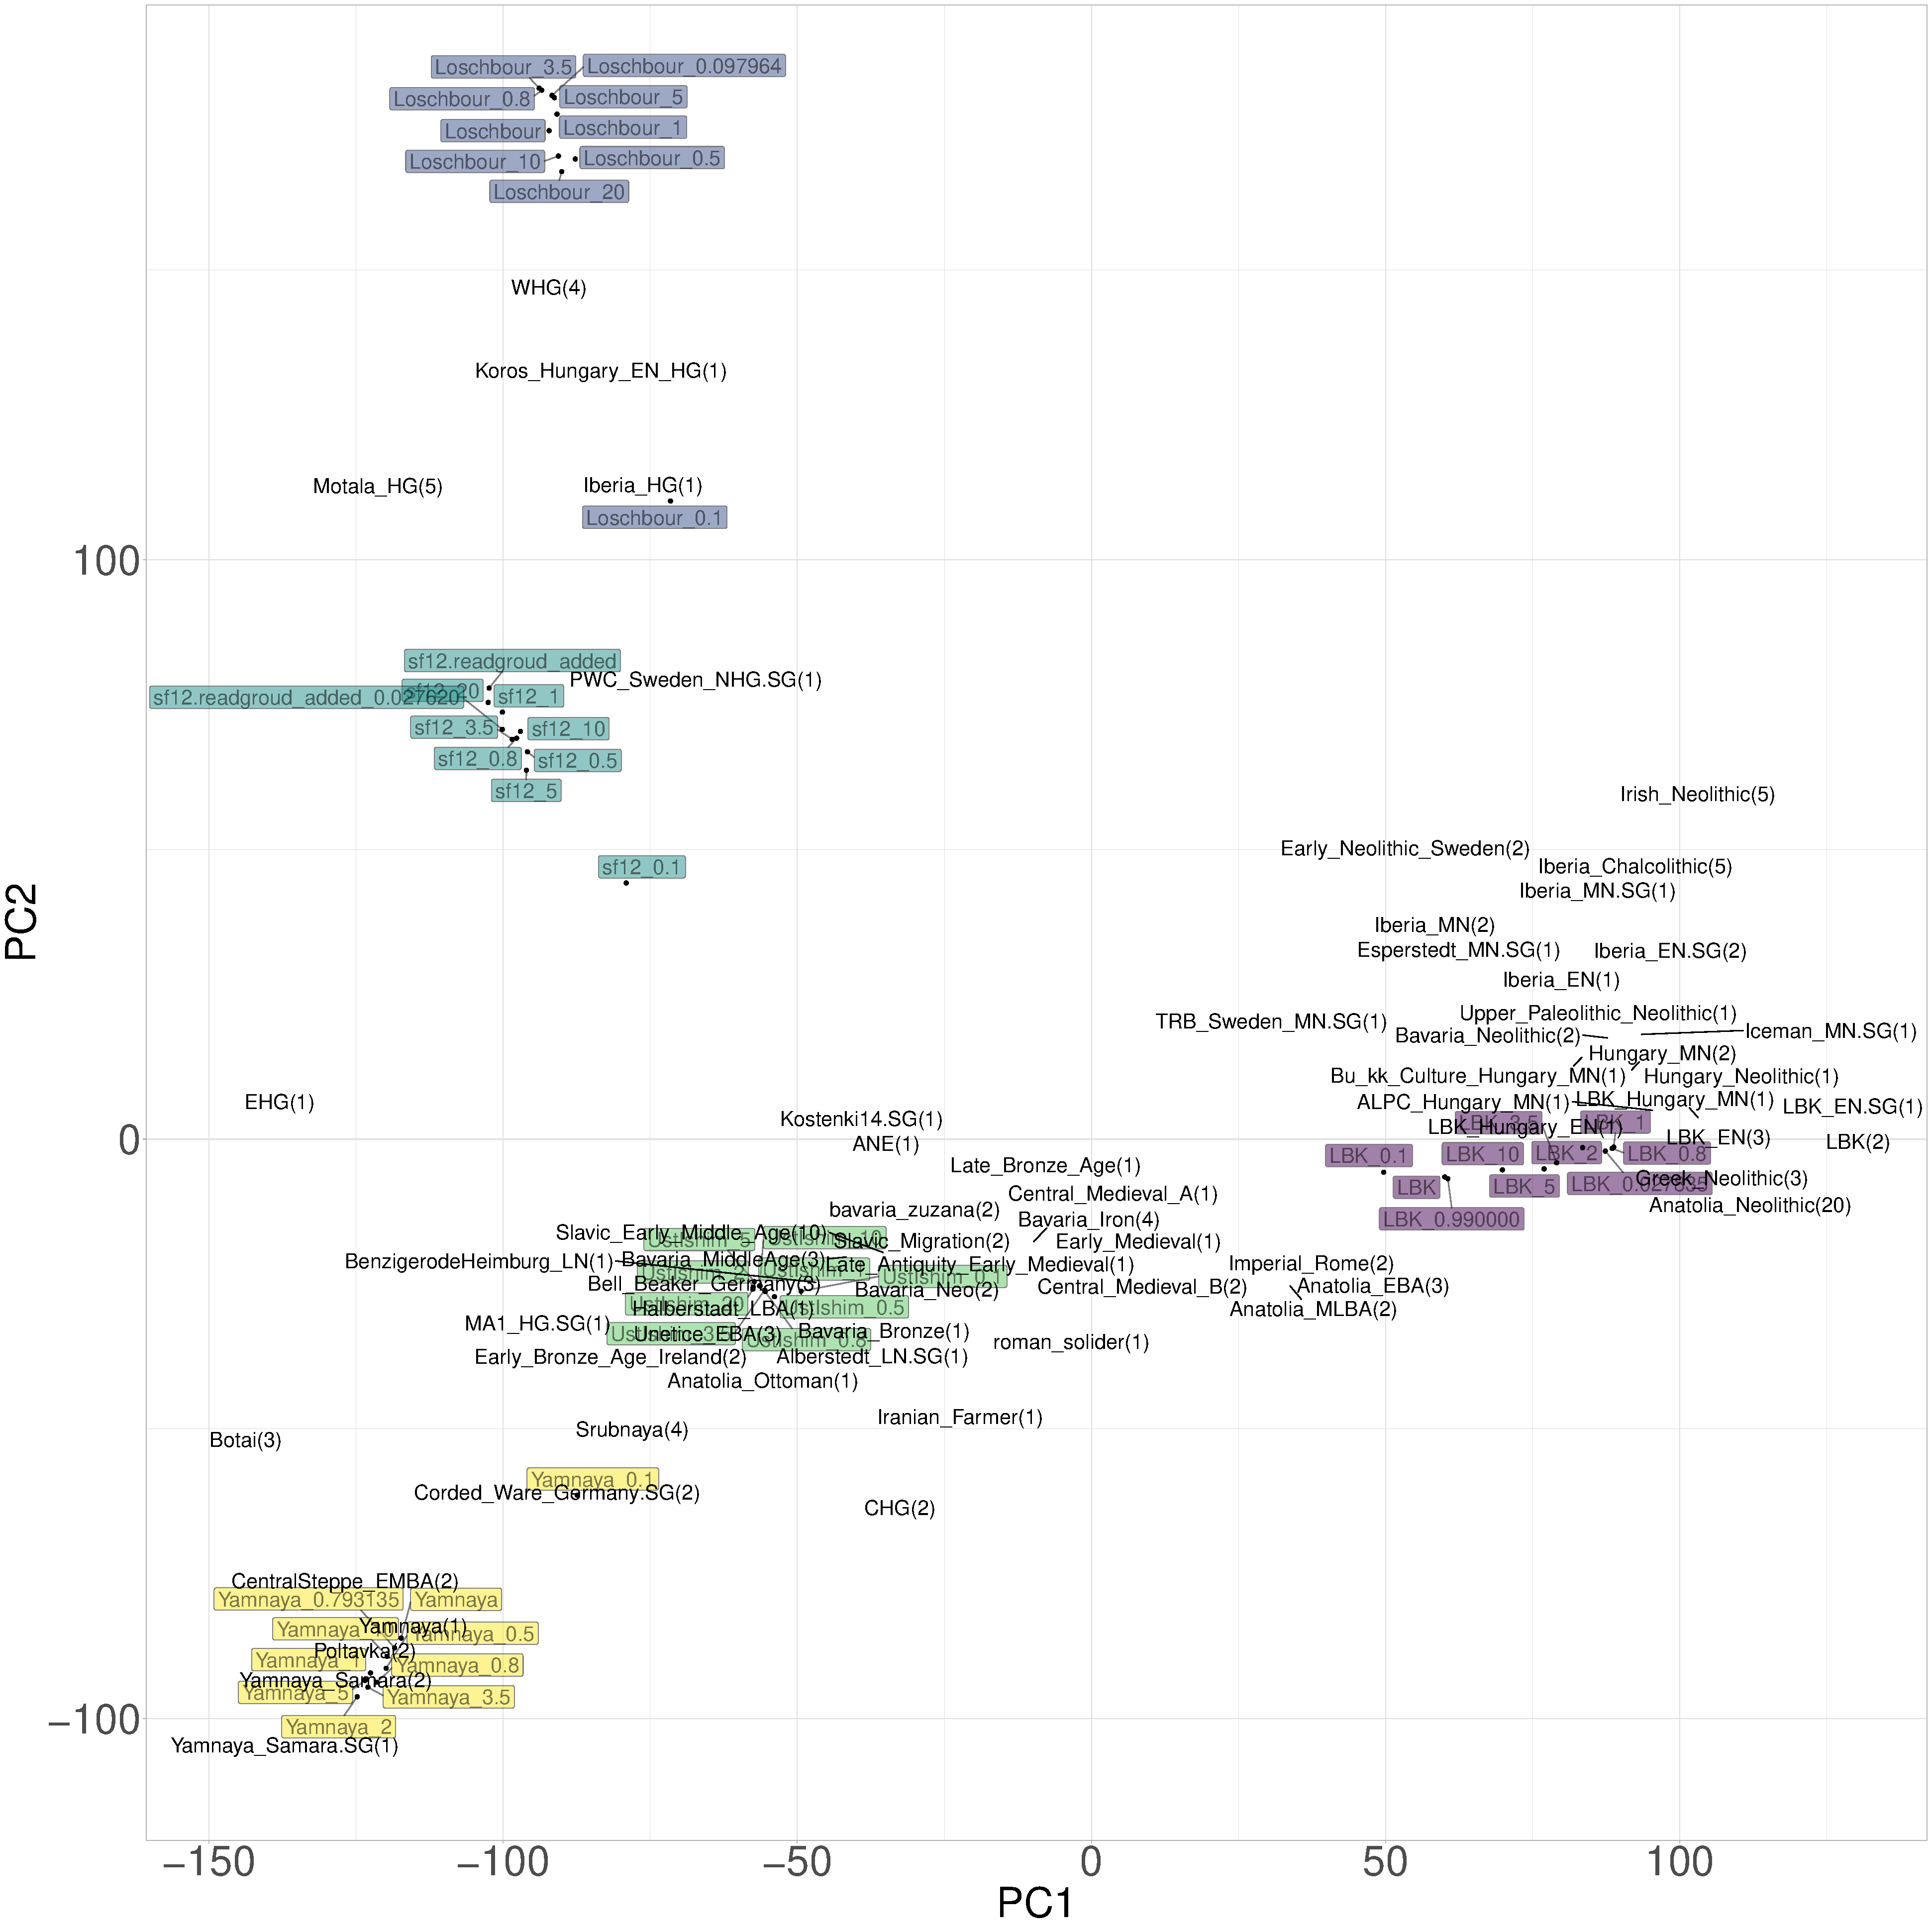
\includegraphics[width=1.0\textwidth]{../images/chapter1/PCA_panel_allInds.allCoverage.pdf}
    \caption{Principle component analysis (PCA) of downsampled, full coverage and downloaded ancient individuals generated from the linked chunklengths matrix. Full coverage and downsampled genomes of the same individual are coloured the same. Reference individuals are grouped into populations plotted as the mean principle components for all individuals within the population. Numbers in labels correspond to the number of individuals within the reference population. 0.1x samples have red border for clarity.}
    \label{fig:PCA_panel_allInds_allCoverage}
\end{figure}

Taken together, these data suggest minimal effect of coverage down to and including 0.5x.

\subsection{SOURCEFIND}

I next determined the effect of sequencing coverage on the ancestry proportions estimated by SOURCEFIND. The chunklengths matrix contains information about the total length of genome one particular individual most closely matches to any other individual. However, this information is often noisy due to phenomena such as incomplete lineage sorting and variable donor group sizes. Therefore, it is often desirable to model out this noise and estimate ancestry proportions in each individual, which are cleaner and more interpretable than raw chunk lengths. 

I began by considering three ancestral sources, or `surrogates', fixed as Anatolia Neolithic, Western Hunter-Gatherer and Yamnaya steppe pastoralist. I compared inferred proportions for the same individual across different levels of coverage (Fig. \ref{fig:3pop_SF_downsampled}). 

\begin{figure}[htp]
    \centering
    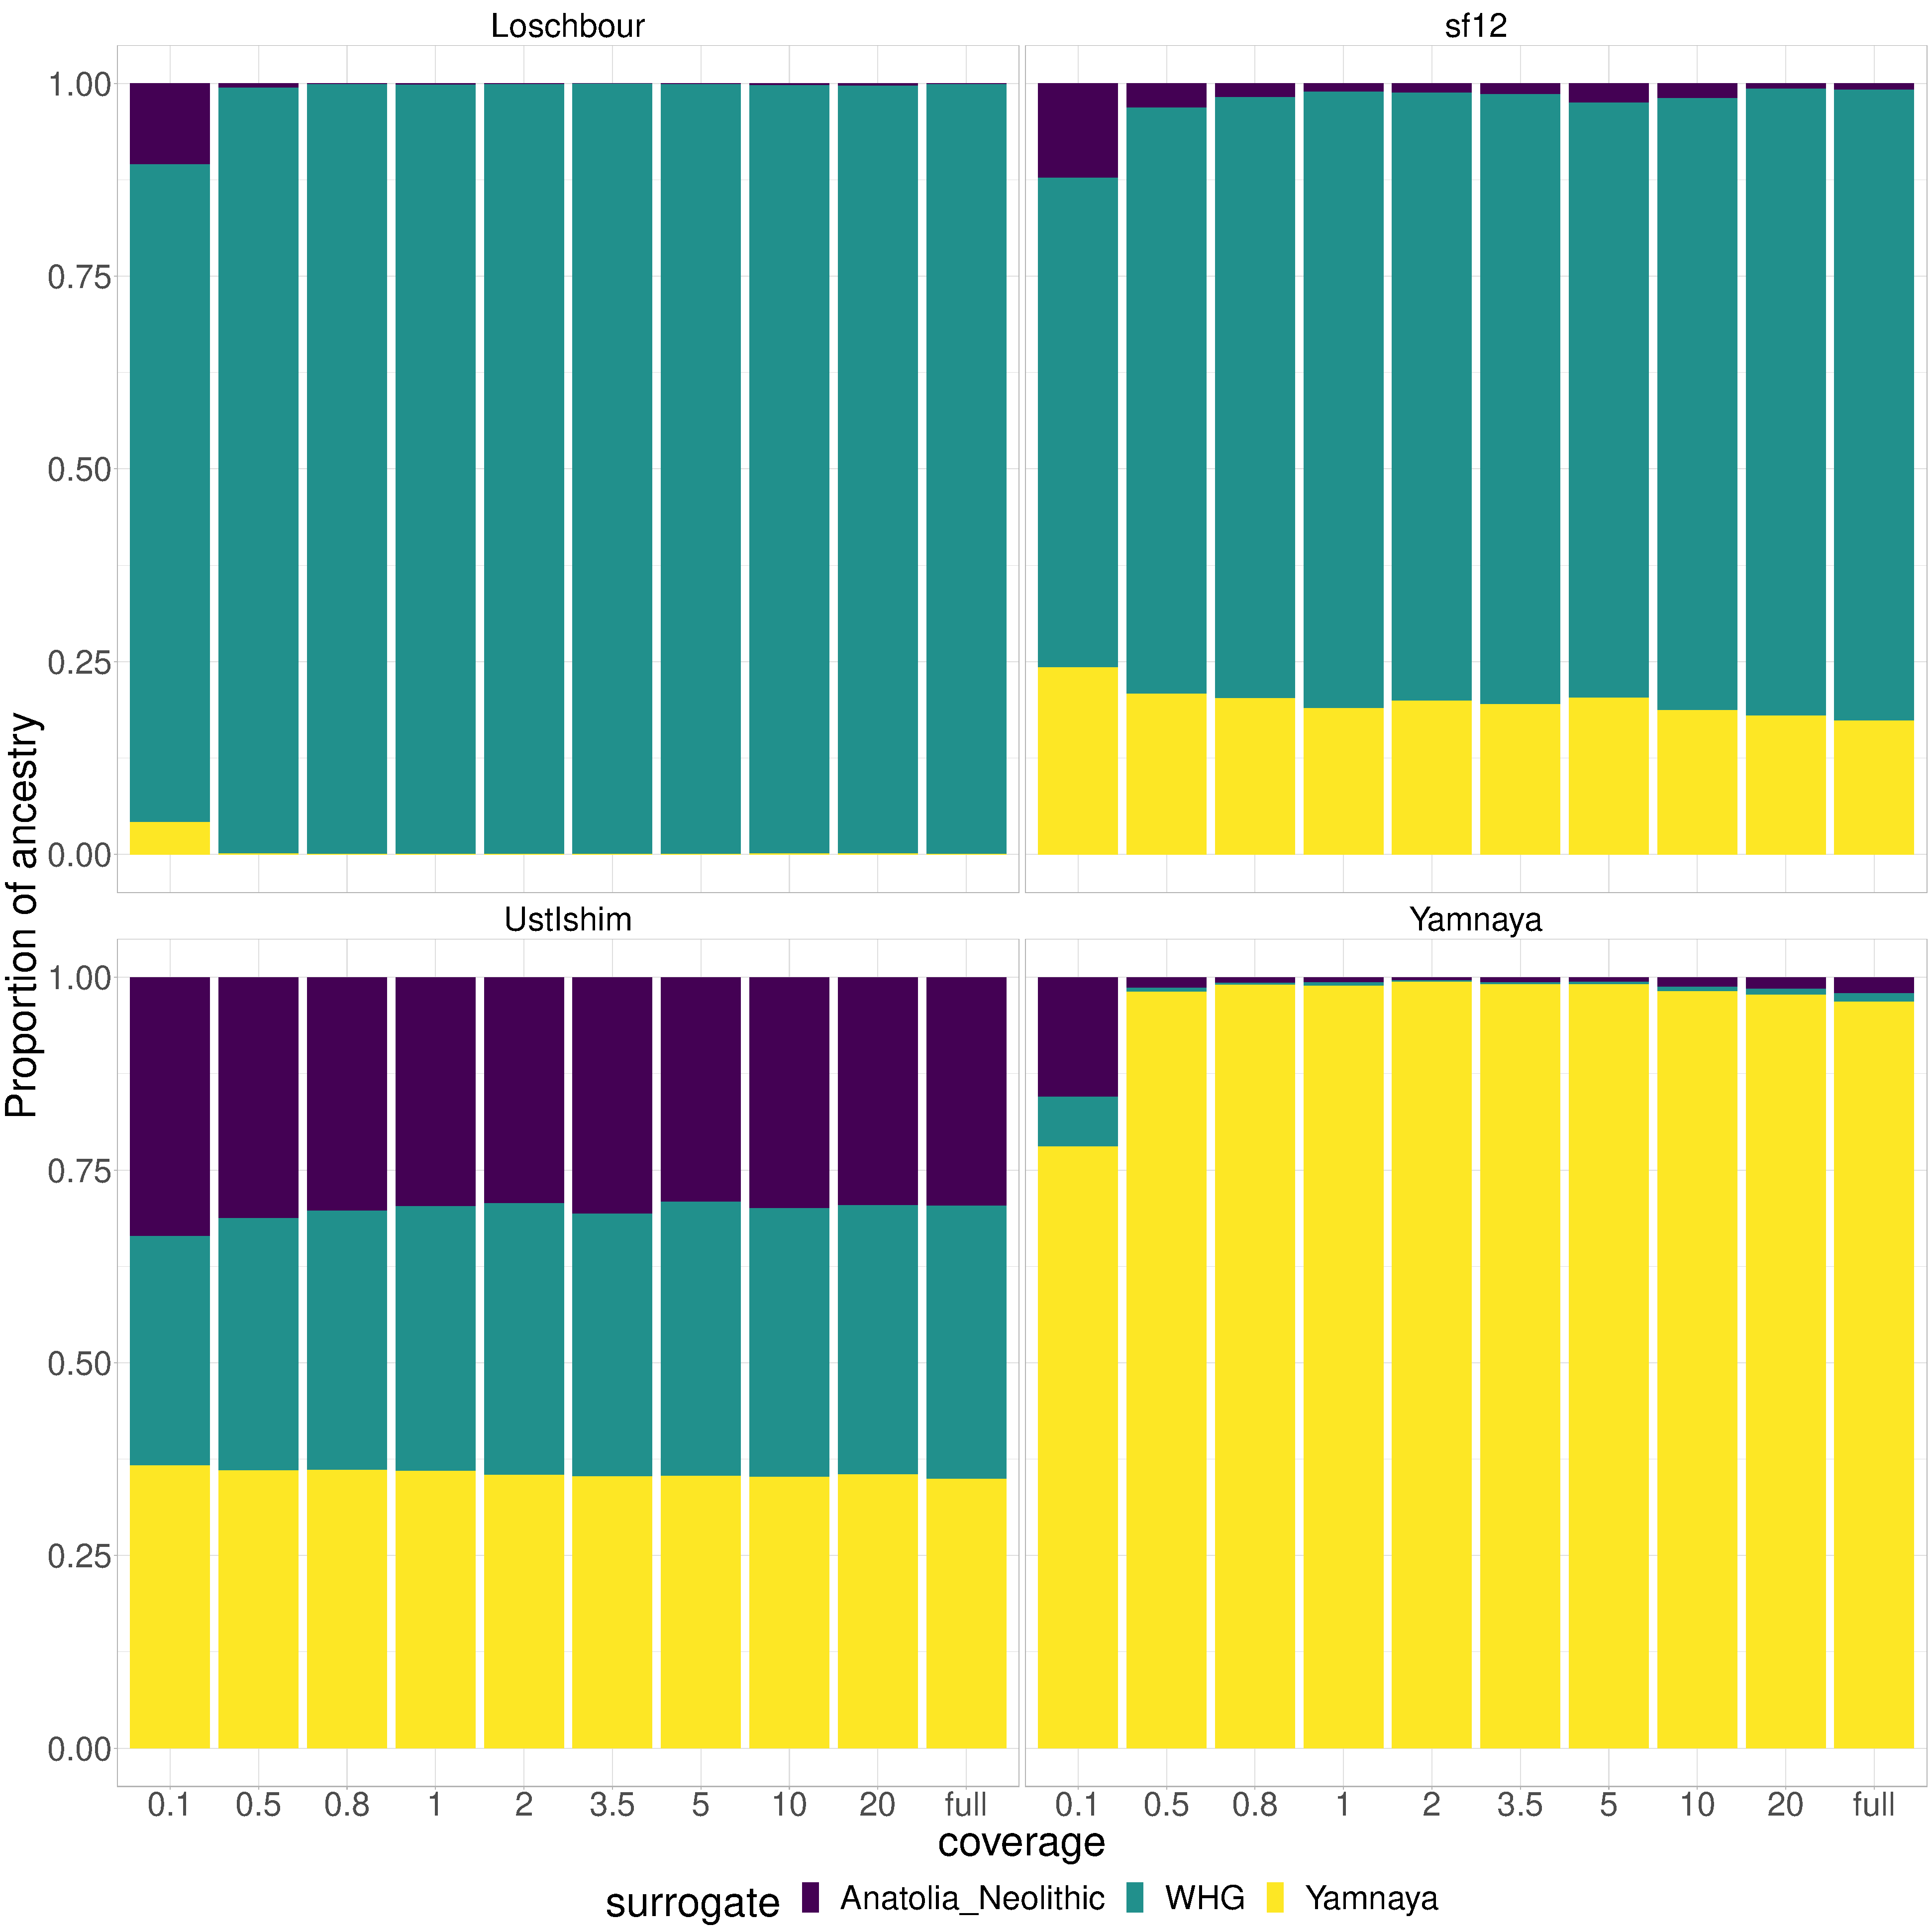
\includegraphics[width=1.0\textwidth]{../images/chapter1/3pop_SF_downsampled.pdf}
    \caption{Each panel gives inferred recent ancestry sharing proportions for a different downsampled genome. Bars represent proportion of ancestry, coloured by different surrogates. Different coverages for the same individual are given within each panel. Three surrogates were used.}
    \label{fig:3pop_SF_downsampled}
\end{figure}

The results suggest that SOURCEFIND estimates are robust down to 0.5-0.8x coverage. At 0.1x coverage, there is an increase in ancestry components that are not present in higher coverage samples, suggesting they are artifacts caused by low coverage. For example, small components of Anatolia Neolithic and Yamnaya ancestry appear in Loschbour at 0.1x coverage, which are not present at any higher coverages. Above 0.5x coverage, the effect of coverage on estimated ancestry proportions appears to be marginal. For example, in sf12, the difference in the minor ancestry component of Anatolia Neolithic is, at most, 2.369\%.

However, more than three surrogates are often used, as SOURCEFIND is meant to infer the most important contributors without a priori knowledge of the samples' ancestry. Therefore, I re-ran SOURCEFIND using 39 surrogate populations. A strength of SOURCEFIND is that many surrogate populations can be used; unlike qpAdm or ADMIXTURE, {\color{red}where a reduced set must be used (reword this and get some evidence)[YES -- I THINK IN THEORY qpAdm CAN USE MULTIPLE SURROGATES]} (Fig. \ref{fig:SOURCEFIND_AllPSop_downsampled}). 

\begin{figure}[htp]
    \centering
    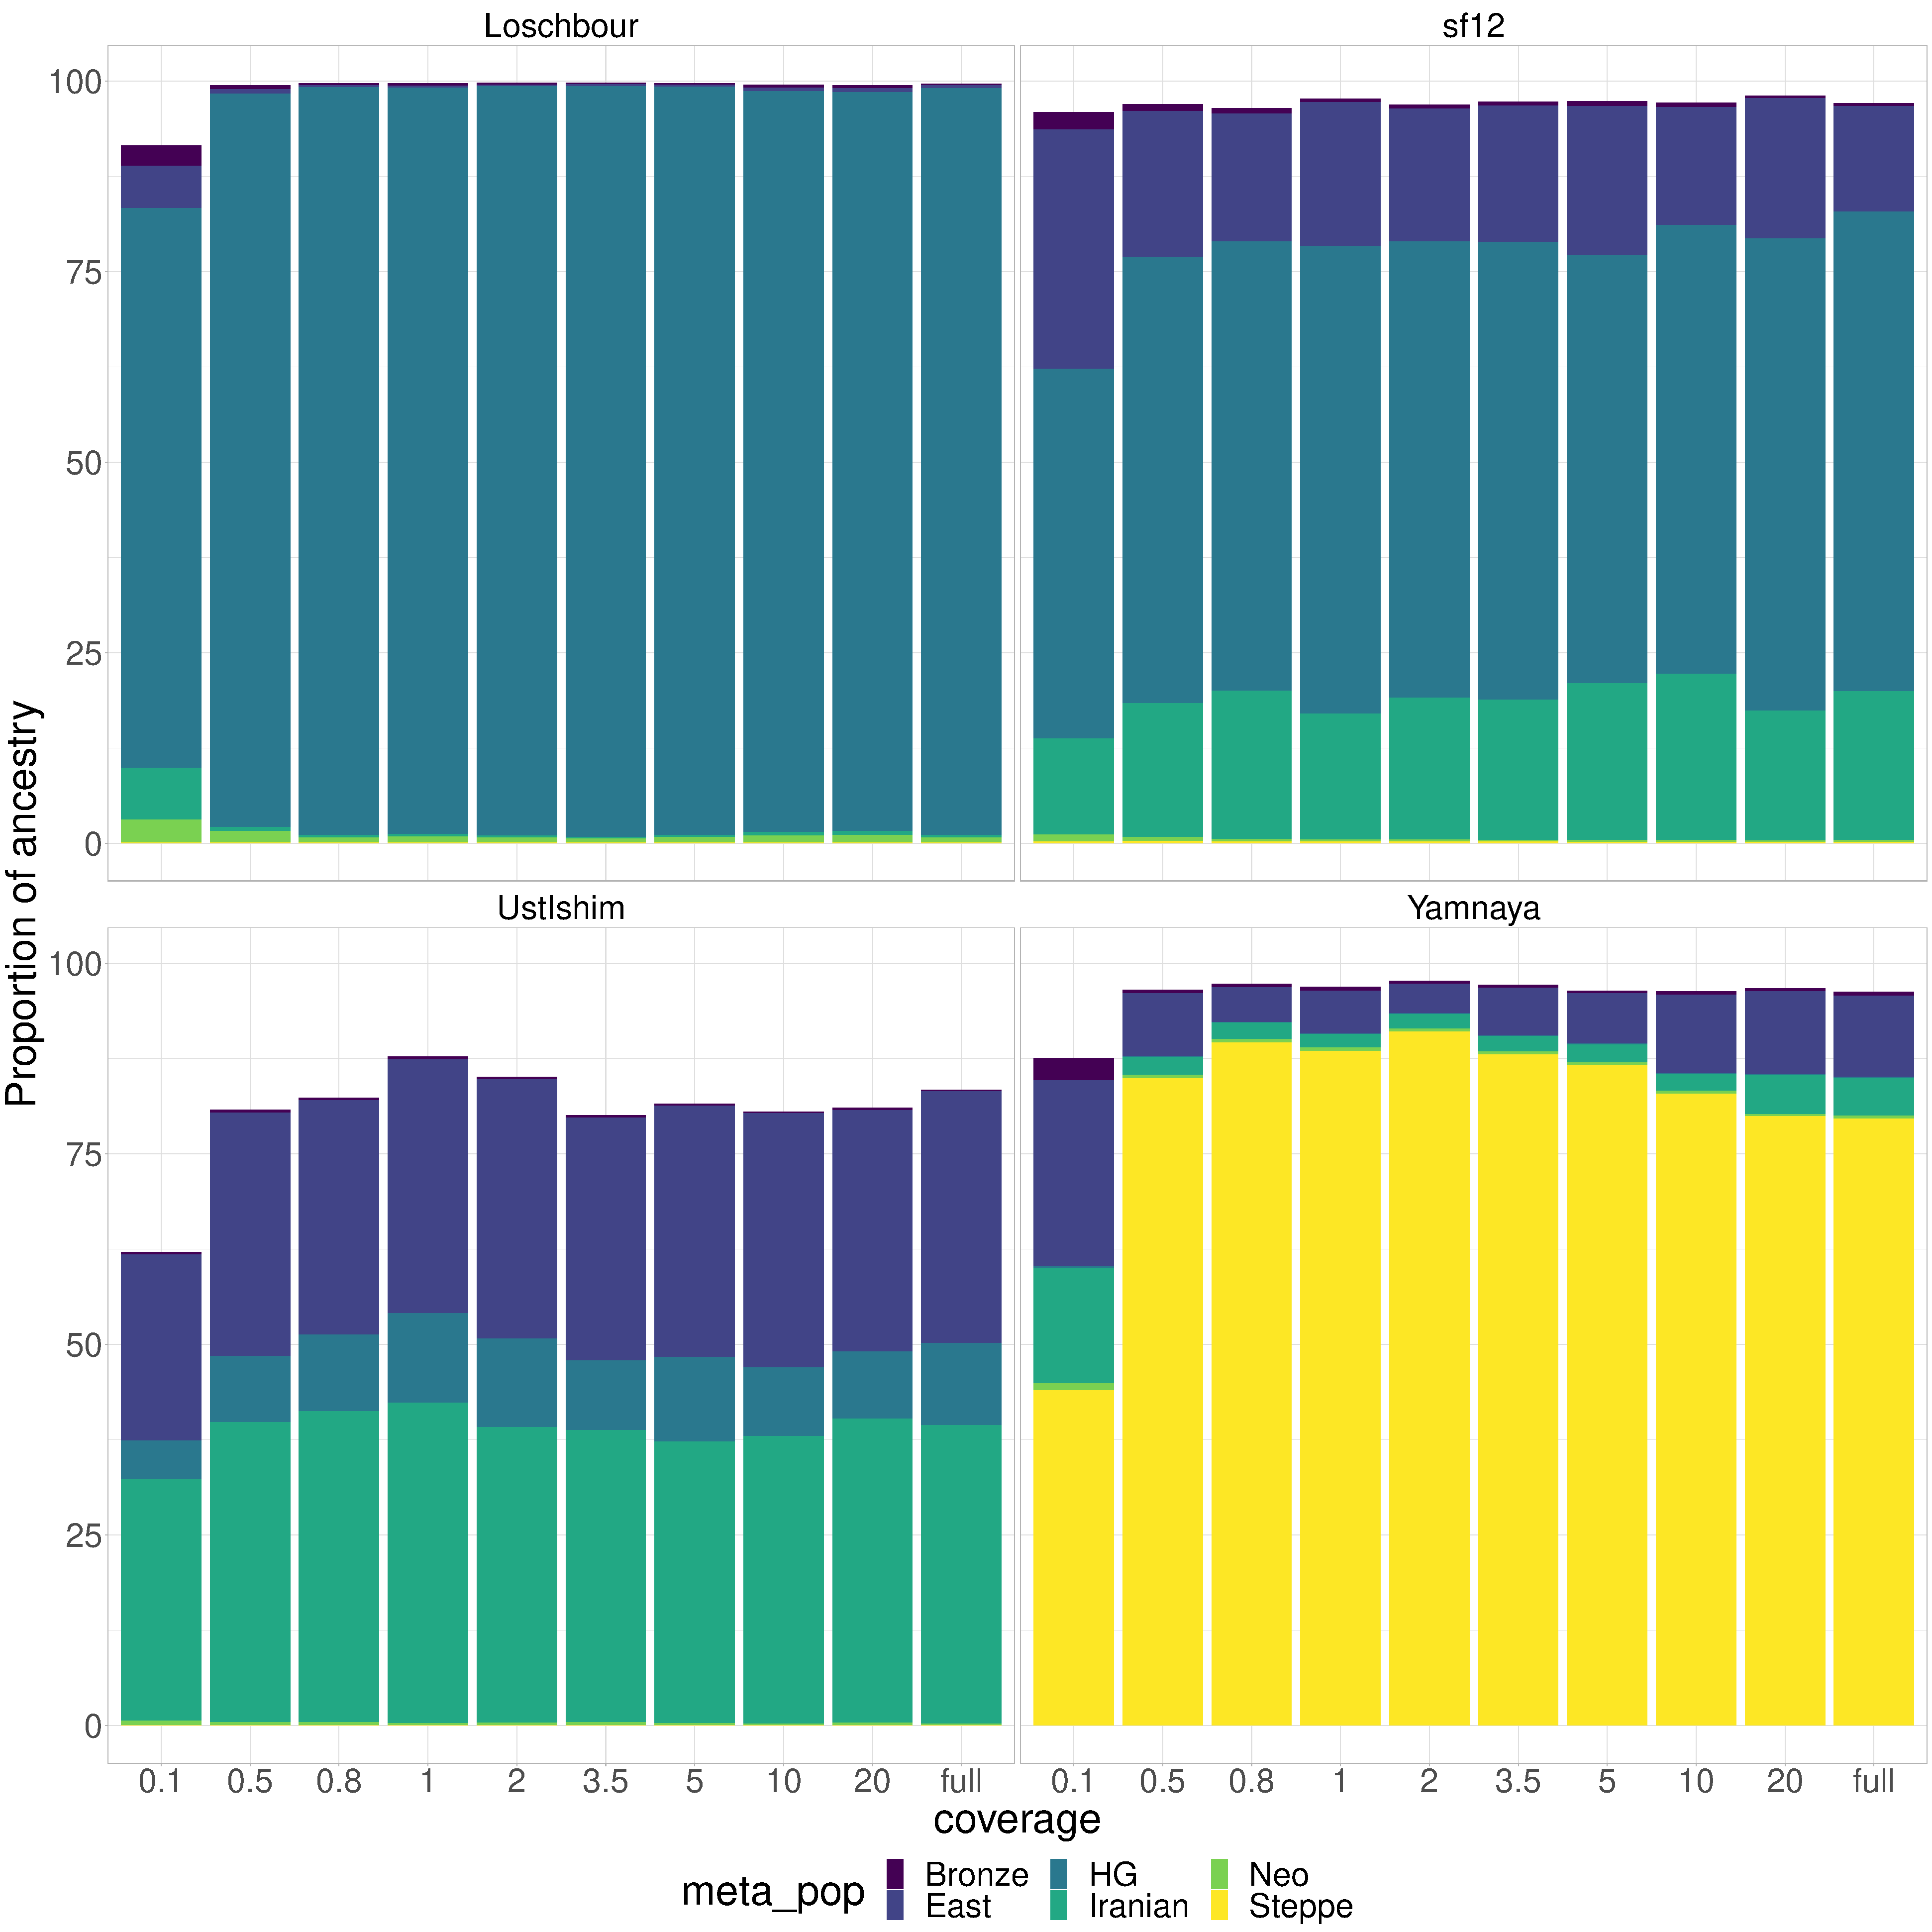
\includegraphics[width=1.0\textwidth]{../images/chapter1/Allpops_SF_downsampled.pdf}
    \caption{Each panel gives information for a different downsampled genome. Bars represent proportion of ancestry, coloured by different surrogates. Different coverages for the same individual are given within each panel. All 39 ancient surrogates were used. Only surrogates with more than 5\% are shown. {\color{red}[ONE OPTION MIGHT BE TO COLOR ONLY \{Ana\_Neo,WHG,Yamnaya\} AS IN FIG 2.9, THOUGH SF12 WILL BE ODD. CAN YOU SOMEHOW CATEGORISE THE SURROGATES INTO HOW THEY FALL INTO THOSE THREE FIG 2.9 CATEGORIES?]}}
    \label{fig:SOURCEFIND_AllPSop_downsampled}
\end{figure}

Again, Loschbour seems to be the least affected by coverage, with only slight differences between the 0.5x and full coverage samples. It is known that Upper Paleolithic / Early Neolithic Hunter-Gatherer populations were small and lacked genetic diversity \cite{excoffier1999hunter, Lazaridis2014, Fu2016}. It is therefore expected that Hunter-Gatherers would share longer IBD segments than individuals from outbred populations. Accordingly, this may make estimating SOURCEFIND proportions easier.


\section{Issues and possible solutions for low coverage ancient DNA}

The previous section outlined a drawback of performing ChromoPainter analysis on low coverage (less than 0.5x) ancient DNA samples; low coverage samples appear to be shifted towards the origin of a principle component analysis (PCA) relative to the same sample at higher coverage (Fig. \ref{fig:PCA_panel_allInds_allCoverage}). This is evident for the lowest coverage samples at 0.1x and suggests that samples of this coverage cannot be reliably analysed using         current methodology.

In order to solve the issue of coverage-related bias, it is first necessary to determine at which stage of the analysis pipeline this bias is introduced. By `analysis pipeline', I refer to the stages of variant calling, imputation and phasing, and ChromoPainter described in the methods section.

\subsection{PCA imputation test}

To explicitly test at what stage the bias is introduced, I performed a set of principle component analyses on the downsampled data. First, I performed PCA projections of all downsampled ancient individuals onto a set of present-day European individuals using i) pre-GLIMPSE genotypes and ii) post-GLIMPSE (imputed) genotypes (Fig. \ref{fig:pre_GLIMPSE_PCA}). PCA projections are used when the target dataset, in this case downsampled ancients, contain variable levels of missing data.  

The results show that there is no apparent coverage-related bias in the pre-GLIMPSE PCA; the 0.1x samples do not substantially differ in their position from the other downsamples of the same individual. However, there is a degree of noise; for example, the LBK downsamples are spread over a small region on the PCA. 

On the other hand, the 0.1x samples are clearly shifted to the centre of the post-GLIMPSE PCA, away from the full coverage individual and other downsamples. This suggests that coverage-related bias is being introduced in the imputation stage. GLIMPSE appears to have removed some of the noise in the downsampled individuals. For instance, the noise observed in the LBK samples in the pre-imputation PCA is substantially reduced and the samples cluster more tightly.  

I also performed a PCA, using the same set of present-day European samples and downsampled ancient individuals as previously, but on the chunklengths matrix ChromoPainter output. There is an increased amount of noise and evidence of coverage-related bias relative to the post-GLIMPSE genotype PCA. Fig. \ref{fig:pre_GLIMPSE_PCA}) displays the PCA for the same painting, but using the unlinked chunkcounts matrix. Comparing the linked and unlinked PCAs shows the effect of including linkage (i.e. haplotype information) on the amount of bias and noise across each sample. Per-sample, there is reduced noise in the unlinked painting.

These results suggest that imputation introduces a degree of bias into 0.1x samples that is not apparent on non-imputed genotypes. They also suggest that ChromoPainter introduces an additional degree of bias, or that it amplifies bias already present introduced at the imputation stage. Accordingly, removing SNPs which have been poorly imputed may be a way to mitigate such biases.

\begin{figure}[htp]
    \centering
    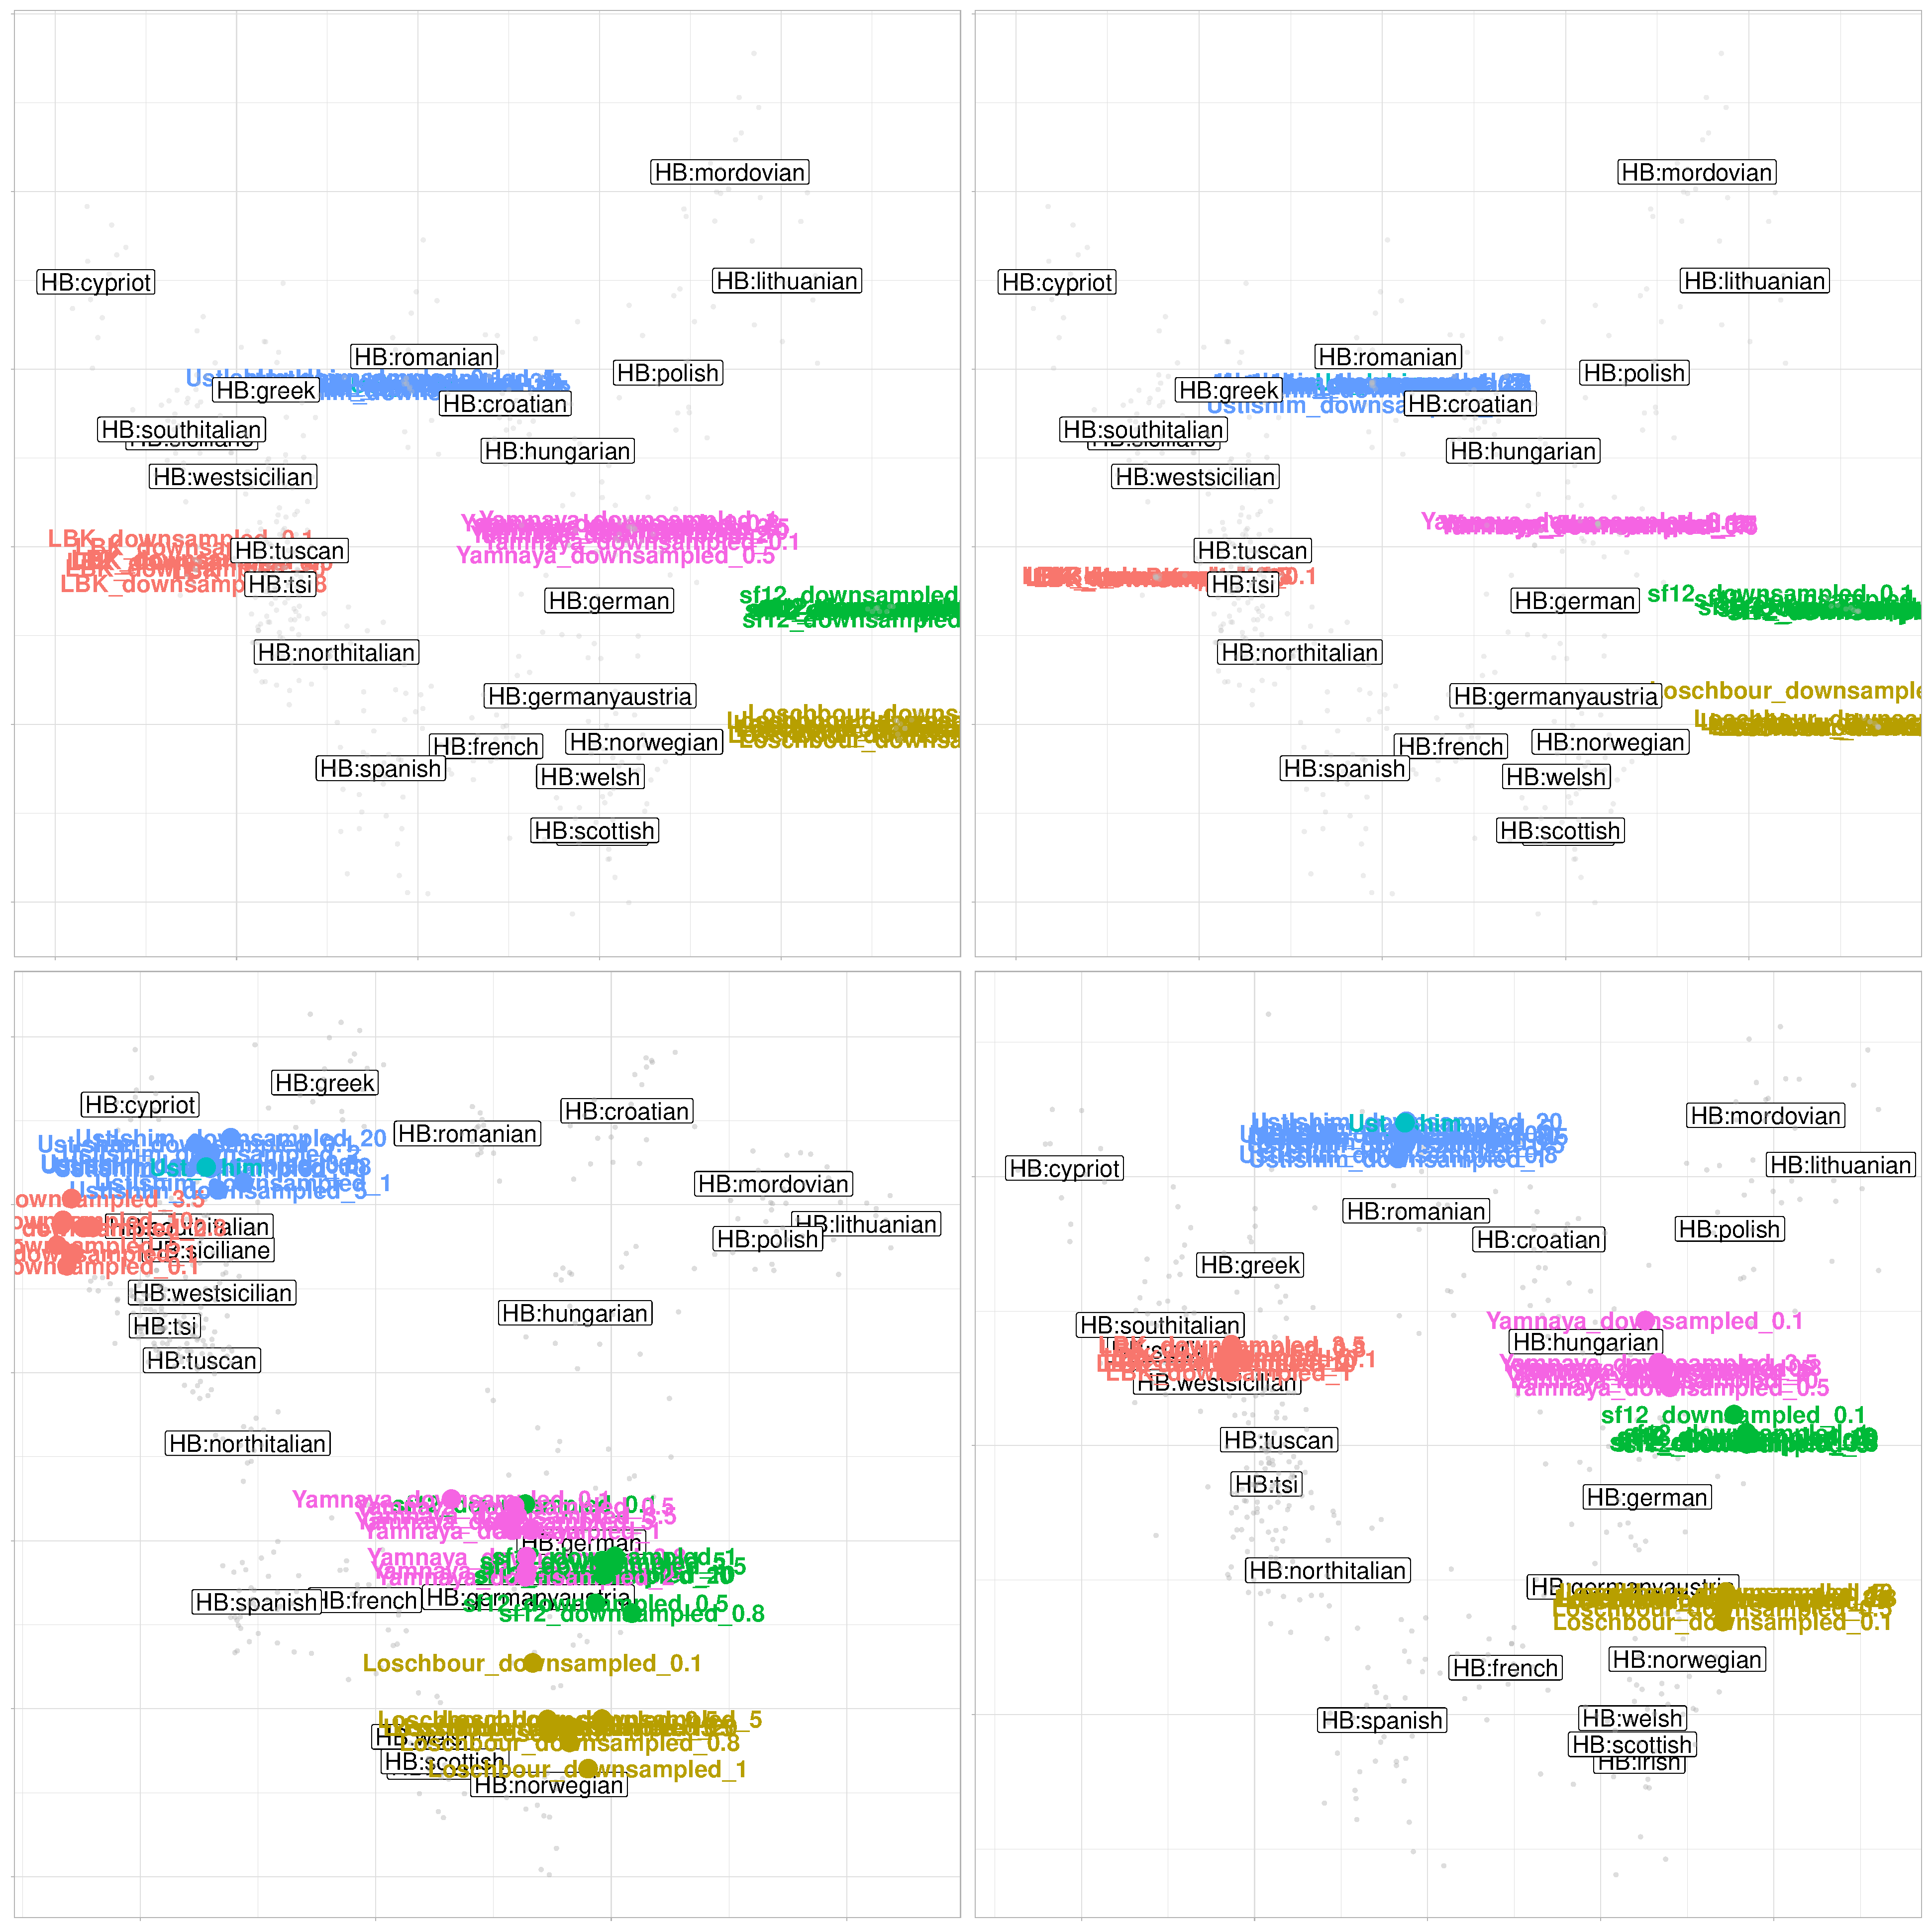
\includegraphics[width=1.0\textwidth]{../images/chapter1/CP_linked_unlinked_pre_post_GLIMPSE_PCA.pdf}
    \caption{Principle Component Analysis. Top Left - pre-GLIMPSE genotypes. Top Right - post-GLIMPSE genotypes. Bottom Left - ChromoPainter Linked. Bottom-Right - ChromoPainter Unlinked. White labels correspond to the midpoint of all samples from that population, grey points correspond to modern individuals.}
    \label{fig:pre_GLIMPSE_PCA}
\end{figure}

\subsection{Direct imputation test} \label{DirectImputationTest}

The previous section suggested that imputation plays a role in the introduction of coverage-related bias. However, it is not clear whether it is `bias', i.e.\ towards the reference population used to assist imputation, or `noise' due to random incorrect imputation. To directly test whether the effect of imputation is noise or bias, I used the Human Origins dataset (described in appendix A.19), containing the genotypes of 5998 present-day individuals from across the world, genotyped at 560,442 SNPs. I chose to use present-day samples because there is a larger total number of individuals and larger number of individuals per population. Additionally, the populations in present-day samples are more homogenous and well-defined. compared to ancient groups. I set all but 70,000 SNPs as missing and imputed missing positions using the HRC as a reference, in order to simulate a dataset where the majority of SNPs are imputed. I then performed an all-v-all painting of i) the original Human Origins dataset where none of the 560,442 SNPs had been imputed and ii) the simulated dataset where 430,000 SNPs had been imputed. 

Bias occurs when missing genotypes are incorrectly imputed with variants from certain populations more frequently than others. We might expect these populations to be those which are more prevalent in the reference panel, or from populations closest to the target population. We would correspondingly expect bias to mean that, when painted, some donor populations would donate more than others, relative to if no imputation had taken place. On the other hand, if `noise' is dominating results, we would expect the incorrectly imputed genotypes to be randomly distributed across populations and similarly, we would not expect to see any populations donating more than others relative to if no imputation had taken place. 

Therefore, we can compare the amount different donor groups donate under the imputed and non-imputed SNP set by plotting the mean amount donated by each population using imputed SNPs and non-imputed SNPs (Fig. \ref{fig:imputed_nonimputed_donation}){\color{red}[THIS IS ACROSS ALL RECIPIENTS? ASSUMING THERE ARE SIMILAR NUMBER OF SNPS IN BOTH ANALYSES, IT SEEMS UNCLEAR WHETHER THIS IS B/C HAPLOTYPES ARE CAPTURING MORE (CORRECT) INFORMATION WHEN USING IMPUTATION (E.G.\ B/C IMPUTATION FIXES INCORRECT CALLS). CAN YOU REDO WHILE EXCLUDING ALL EUROPEAN RECIPIENTS? YOU CAN JUST ADD A SENTENCE NOTING RESULTS DON'T CHANGE IF YOU DO SO]}. The 20 populations that contribute most are either European or Jewish. Notably, the Haplotype Reference Consortium panel which was used to imputed the data consists primarily of individuals of European descent. The two populations which are over-copied the most after imputation are two English populations from Kent and Cornwall. 

This suggests that there is a clear bias towards copying more from European populations when the data has been imputed using the HRC. 


\begin{figure}[htp]
    \centering
    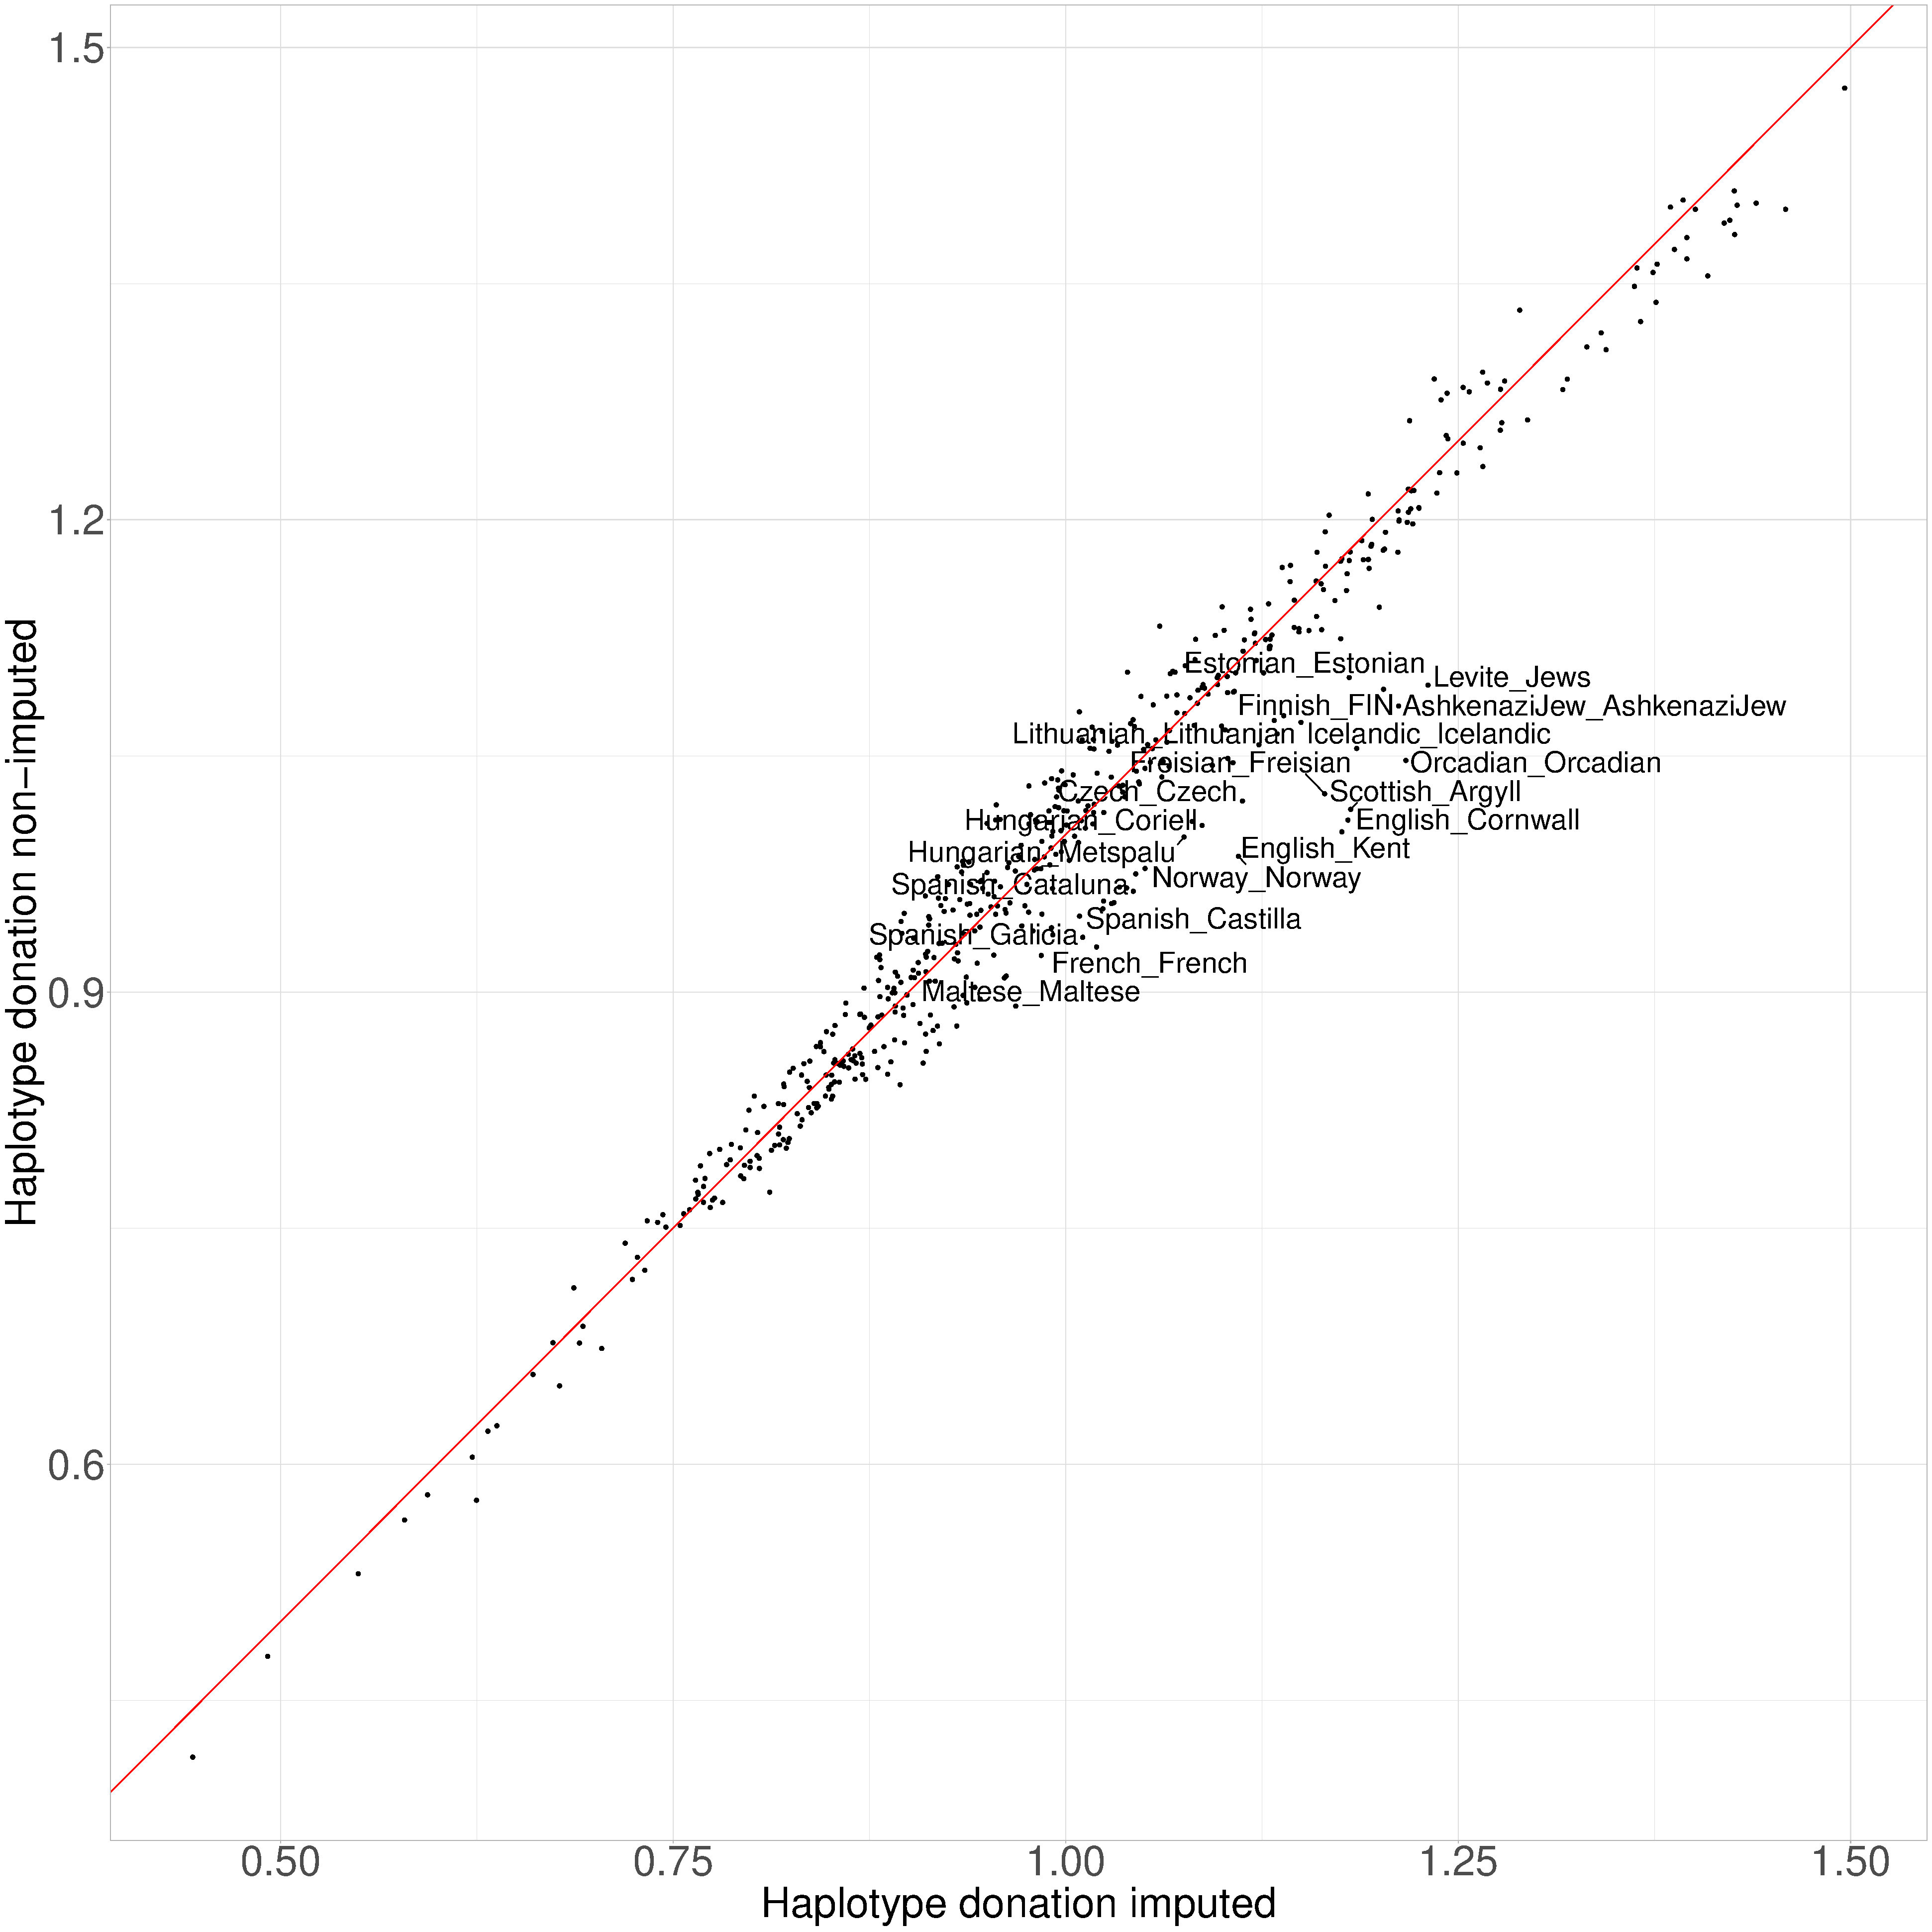
\includegraphics[width=1.0\textwidth]{../images/chapter1/donation_imputed_nonimputed.pdf}
    \caption{Comparison of the mean normalised cM donated by each donor population using the imputed and non-imputed SNP sets. The 20 populations with the largest different between imputed and non-imputed donation are highlighted.}
    \label{fig:imputed_nonimputed_donation}
\end{figure}

\section{Solutions}

In this section I will explore potential solutions to the issue of coverage-related bias. Based on the findings in previous sections, imputation causes bias towards particular reference populations in modern samples.  

\subsection{Accounting for allele likelihoods}

Section 2.2.1 describes an improvement to the ChromoPainter algorithm. Instead of assuming that each allele on a haplotype is correct with a probability $1-\theta$, where $\theta$ represents an error probability, the posterior genotype probability from GLIMPSE is accounted for in the emission probabilities of the copying model. The motivation behind this update is that the uncertainty associated with genotype calls at low coverage is suitably propagated throughout the painting process, resulting in uncertain alleles contributing less towards the expected copying values than more certain ones. This is similar in spirit to that of Viera et al (2016), who account for genotype likelihoods to infer inbreeding IBD tracts from low coverage sequencing data \cite{vieira2016estimating}.

To determine whether accounting for allele likelihoods improved the painting accuracy of a low-coverage genome, I painted the individuals downsampled to 0.1x and 0.5x and corresponding full coverage samples using the `standard set' of ancient reference individuals, using both ChromoPainterV2 and ChromoPainterV2Uncertainty. I then calculated r-squared between the copyvectors of full coverage and downsampled individuals using the two different methods (Fig. \ref{fig:uncertainty_v_noUncertainty_0.5x_0.1x}). This shows that at 0.1x, the ChromoPainterV2 method clearly outperforms ChromoPainterV2Uncertainty across all samples, whereas at 0.5x, the new method marginally outperforms the standard method. Therefore, while accounting for allele likelihoods may improve performance in cases of coverage $\geq$0.5x, which has been shown to still capture some haplotype information, it does not help in cases of coverage of 0.1x where bias problems persist.


\begin{figure}[htp]
    \centering
    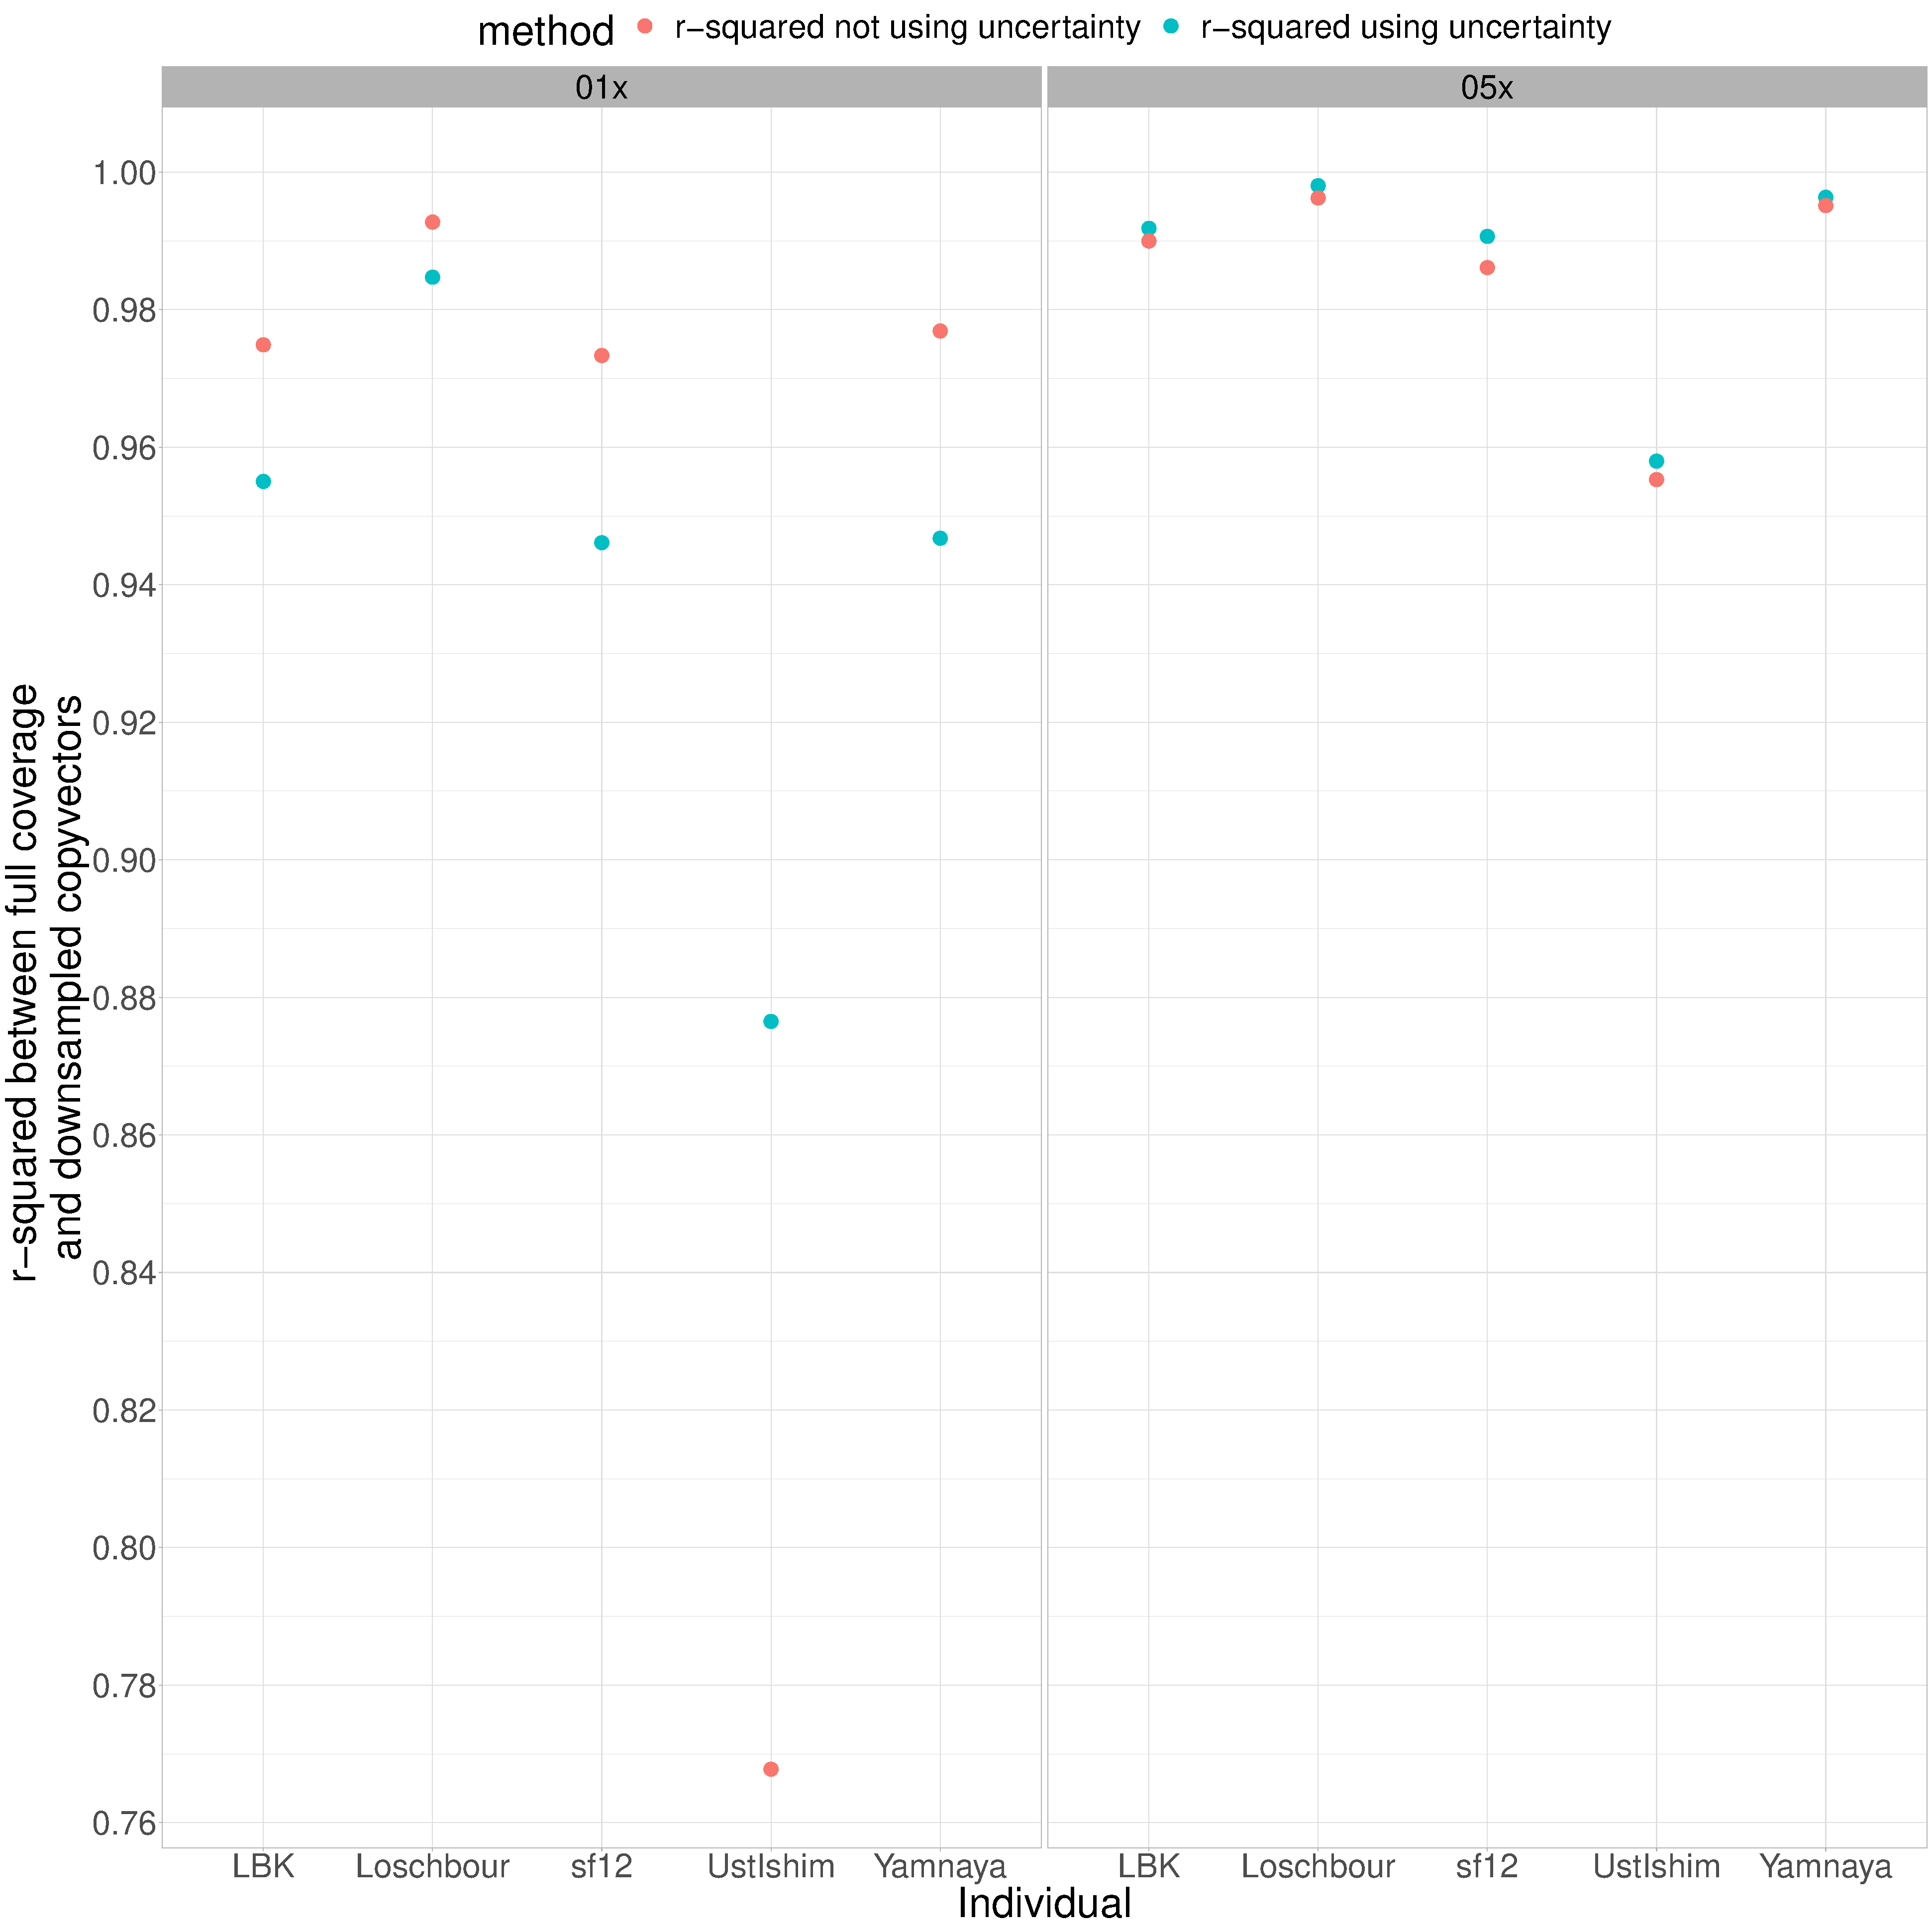
\includegraphics[width=1.0\textwidth]{../images/chapter1/uncertainty_v_noUncertainty_0.5x_0.1x.pdf}
    \caption{Comparison of performance of ChromoPainterV2 and ChromoPainterV2Uncertainty. Panels correspond to samples downsampled to 0.1x (left) and 0.5x (right). Points correspond to the r-squared between the downsampled individual and the same individual at full coverage. Red points are values obtained from ChromoPainterV2 and blue points are those obtained from ChromoPainterV2Uncertainty.}
    \label{fig:uncertainty_v_noUncertainty_0.5x_0.1x}
\end{figure}


\subsection{Filtering SNPs}

In this section, I will test whether filtering the set of input SNPs on different criteria reduces the effect of coverage related bias. 

The frequency of a particular variant in the reference panel (RAF - reference allele frequency) used for imputation is known to affect how accurately that variant can be imputed \cite{rubinacci2021efficient, delaneau2018integrative, Browning2016, hui2020evaluating}. Specifically, we expect variants which are less frequent in the reference panel to be imputed at a lower accuracy than those which are more frequent. Therefore, removing variants with a low frequency in the reference panel may mitigate the coverage related bias by removing variants which have been incorrectly imputed. In other words, we want to retain the SNPs where both alleles are relatively common within the population. 

For each individual, I took the 428,425 SNPs in the HellBus set and removed SNPs with $0.1 > RAF$ or $RAF > 0.9$, removing an average of 50,187 SNPs per individual. $RAF$ refers to the frequency of the allele in the 1000 genomes reference panel used to phase and impute the HellBus I then painted individuals downsampled to 0.1x and 0.5x using the standard set of 125 ancient donor individuals.  

Comparing the r-squared and visually inspecting the relationship between the copvectors showed that this did not improve the 0.5x copyvectors (Fig. \ref{fig:CP_correlation_allSamples_0.1x_0.5x_30x.RAF_filter}{\color{red}[FIGURE MISSING?]}.

I then chose to filter SNPs based on $max(GP)$ at each position. $max(GP)$ correspond to the accuracy with which a SNP has been imputed, with higher values reflecting a higher chance of that genotype being imputed correctly. For each individual downsampled to 0.5x, I only retained positions where the $max(GP) >= 0.990$. This resulted in a total of 348,852 SNPs for LBK, 339,949 for Loschbour, 315,075 for sf12, 308,961 for UstIshim and 386,484 for Yamnaya. Because different SNPs were removed from different individuals, each individual was painted separately. The same standard set of 124 ancient donors was used. Again, this did not improve the accuracy of the copyvectors. 

\begin{table}
\centering
\begin{tabular}[t]{lrrrrrrr}
\toprule
sample & uncertainty\_01x & uncertainty\_05x & standard\_01x & standard\_05x & raf\_01x & raf\_05x & gp\_05x\\
\midrule
LBK & 0.989 & 0.996 & 0.989 & 0.996 & 0.979 & 0.997 & 0.992\\
Loschbour & 0.998 & 0.999 & 0.998 & 0.999 & 0.992 & 0.999 & 0.994\\
sf12 & 0.989 & 0.995 & 0.989 & 0.995 & 0.974 & 0.995 & 0.982\\
Yamnaya & 0.990 & 0.999 & 0.990 & 0.999 & 0.972 & 0.998 & 0.995\\
UstIshim & 0.848 & 0.992 & 0.848 & 0.992 & 0.930 & 0.979 & 0.969\\
\bottomrule
\end{tabular}
\caption{Table of r-squared values between the copyvectors of full coverage and downsampled individuals. `uncertainty' refers to ChromoPainterUncertainty, `standard' refers to ChromoPainterV2, RAF refers to filtering SNPs with reference allele frequency (RAF) $0.1 > RAF$ or $RAF > 0.9$ and `GP' refers to filtering $max(GP) >= 0.990$. [SAM: sorry this has gone off the edge - tried to fix it, but it was causing a lot of issues.{\color{red}[CAN USE longtable INSTEAD. OR USE ``U'' FOR ``uncertainty'', ETC.]}]}
\end{table}



\subsection{Upweighting densely genotype regions of high coverage}

Section \nameref{DirectImputationTest} showed that imputation error was the likely cause of coverage related bias. Thus, restricting analysis to non-imputed SNPs above a certain coverage may mitigate coverage-related bias.

However, reducing the total number and or density of SNPs used in a painting may reduce the accuracy of the estimated copyvectors. All other things being equal, there is less linkage information between two SNPs which are separated by a larger genetic distance. Therefore, it is necessary to precisely determine what effect reducing the number of SNPs has in order to determine whether removing SNPs is a viable strategy. In particular, it is necessary to know the minimum number and density of SNPs required to retain the advantages of haplotype-based methods over unlinked methods. Additionally, it is also important to know whether low-coverage samples have enough SNPs of adequate quality to retain haplotype-information. As haplotype-based methods work by considering contiguous chunks of SNPs, we can ask whether samples of a particular coverage have enough windows of high-quality SNPs to match the power of a high coverage sample.

Previous studies have shown it is possible to distinguish between individuals from Devon and Cornwall using the fineSTRUCTURE clustering algorithm, but not using unlinked methods (ADMIXTURE \cite{alexander2009fast}) \cite{Leslie2015}. Therefore, determining whether it is possible to distinguish between individuals from Devon and Cornwall acts as a good test case for reducing SNPs; how many SNPs can we remove before we lose the ability to distinguish between these two populations?

To test the effect of reducing the number of SNPS, I first painted individuals from Devon and Cornwall with all other POBI populations as donors, using the full set of SNPs (n=452,592) and a reduced set of SNPs, retaining from between 0.2\% - 90\% of the original number of SNPs (a full list of the 12 reduction levels and details of the painting procedure can be found in the methods section).

For the painting containing the full set of SNPs, I estimated the median length of haplotypes donated from POBI counties to individuals in Devon and Cornwall, yielding a value of approximately 500Kb.

Next, I wanted to determine the minimum number of 500Kb windows needed to match the power of the full set of SNPs. To do this, for each level of reducing SNPs, I painted each individual from Devon and Cornwall using all other POBI individuals. Then, for each level of reducing SNPs, I used TVD to assign recipient individual from Devon or Cornwall to either Devon or Cornwall, or in other words, seeing if we could correctly identify the population of origin for the recipient individuals. Beginning with chromosome 22, for each individual, I calculated the TVD with the mean copyvectors of all other recipients from Devon and Cornwall, taking the minimum as the assigned population. I then added in chromosome 21, and assigned the individuals again. I continued to add chromosomes until the power to assign individuals was the same as when using the full set of 500,000 SNPs. Accordingly, for each level of reducing SNPs, I had the chromosomes required to match the power in the full set of SNPs. I converted this value to the total number of non-overlapping 250Kb, 500Kb or 1Mb windows.

We can also estimate, for each level of reducing SNPs and window size, how many `good' SNPs are needed within each window. 500Kb corresponds to 6,000 windows genome-wide. 20\% density is approximately 100,000 SNPs; so 100000/6000 = 16.7 good SNPs are required per window. 

\begin{table}
\centering
\begin{tabular}[t]{lrrr}
\toprule
n\_snps & 250Kb & 500Kb & 1Mb\\
\midrule
40,000 & 7691 & 3879 & 1967\\
45,000 & 6272 & 3166 & 1607\\
50,000 & 5659 & 2858 & 1452\\
100,000 & 3602 & 1820 & 925\\
150,000 & 4083 & 2064 & 1049\\
200,000 & 4083 & 2064 & 1049\\
250,000 & 4083 & 2064 & 1049\\
300,000 & 5659 & 2858 & 1452\\
350,000 & 4507 & 2278 & 1158\\
400,000 & 4083 & 2064 & 1049\\
450,000 & 4083 & 2064 & 1049\\
\bottomrule
\end{tabular}
\caption{Number of 250Kb, 500Kb or 1Mb windows required at different levels of SNP reduction to match the TVD assignment power of 500K fully genotyped SNPs}
\label{table:windows_power_table}
\end{table}

Once I knew the number of windows needed, I searched the genome of each (n=x) ancient individuals for windows of sizes 250Kb, 500Kb or 1Mb for $Y$ SNPs above $Z$ coverage. Then, for each ancient individual in my dataset, I searched in non-overlapping 500Kb windows for Y good SNPs of at least Z coverage (Fig. \ref{fig:avg_good_windows}).

Table \ref{table:windows_power_table} shows that, assuming 100,000 SNPs in total, 2065 windows containing enough at least 16.7 `good' SNPs are required to match the power of full coverage. Fig \ref{fig:avg_good_windows} shows the mean number of good windows per individual at different thresholds of coverage. Circles coloured yellow are above the meet the minimum number of windows requirement. It can be observed that samples less than 0.5x do not have enought windows unless the threshold for `good' SNPs is above 1x coverage. A SNP at 1x coverage has a high probability of missing heterozygous positions. Therefore, these can be excluded. 

\begin{figure}[htp]
    \centering
    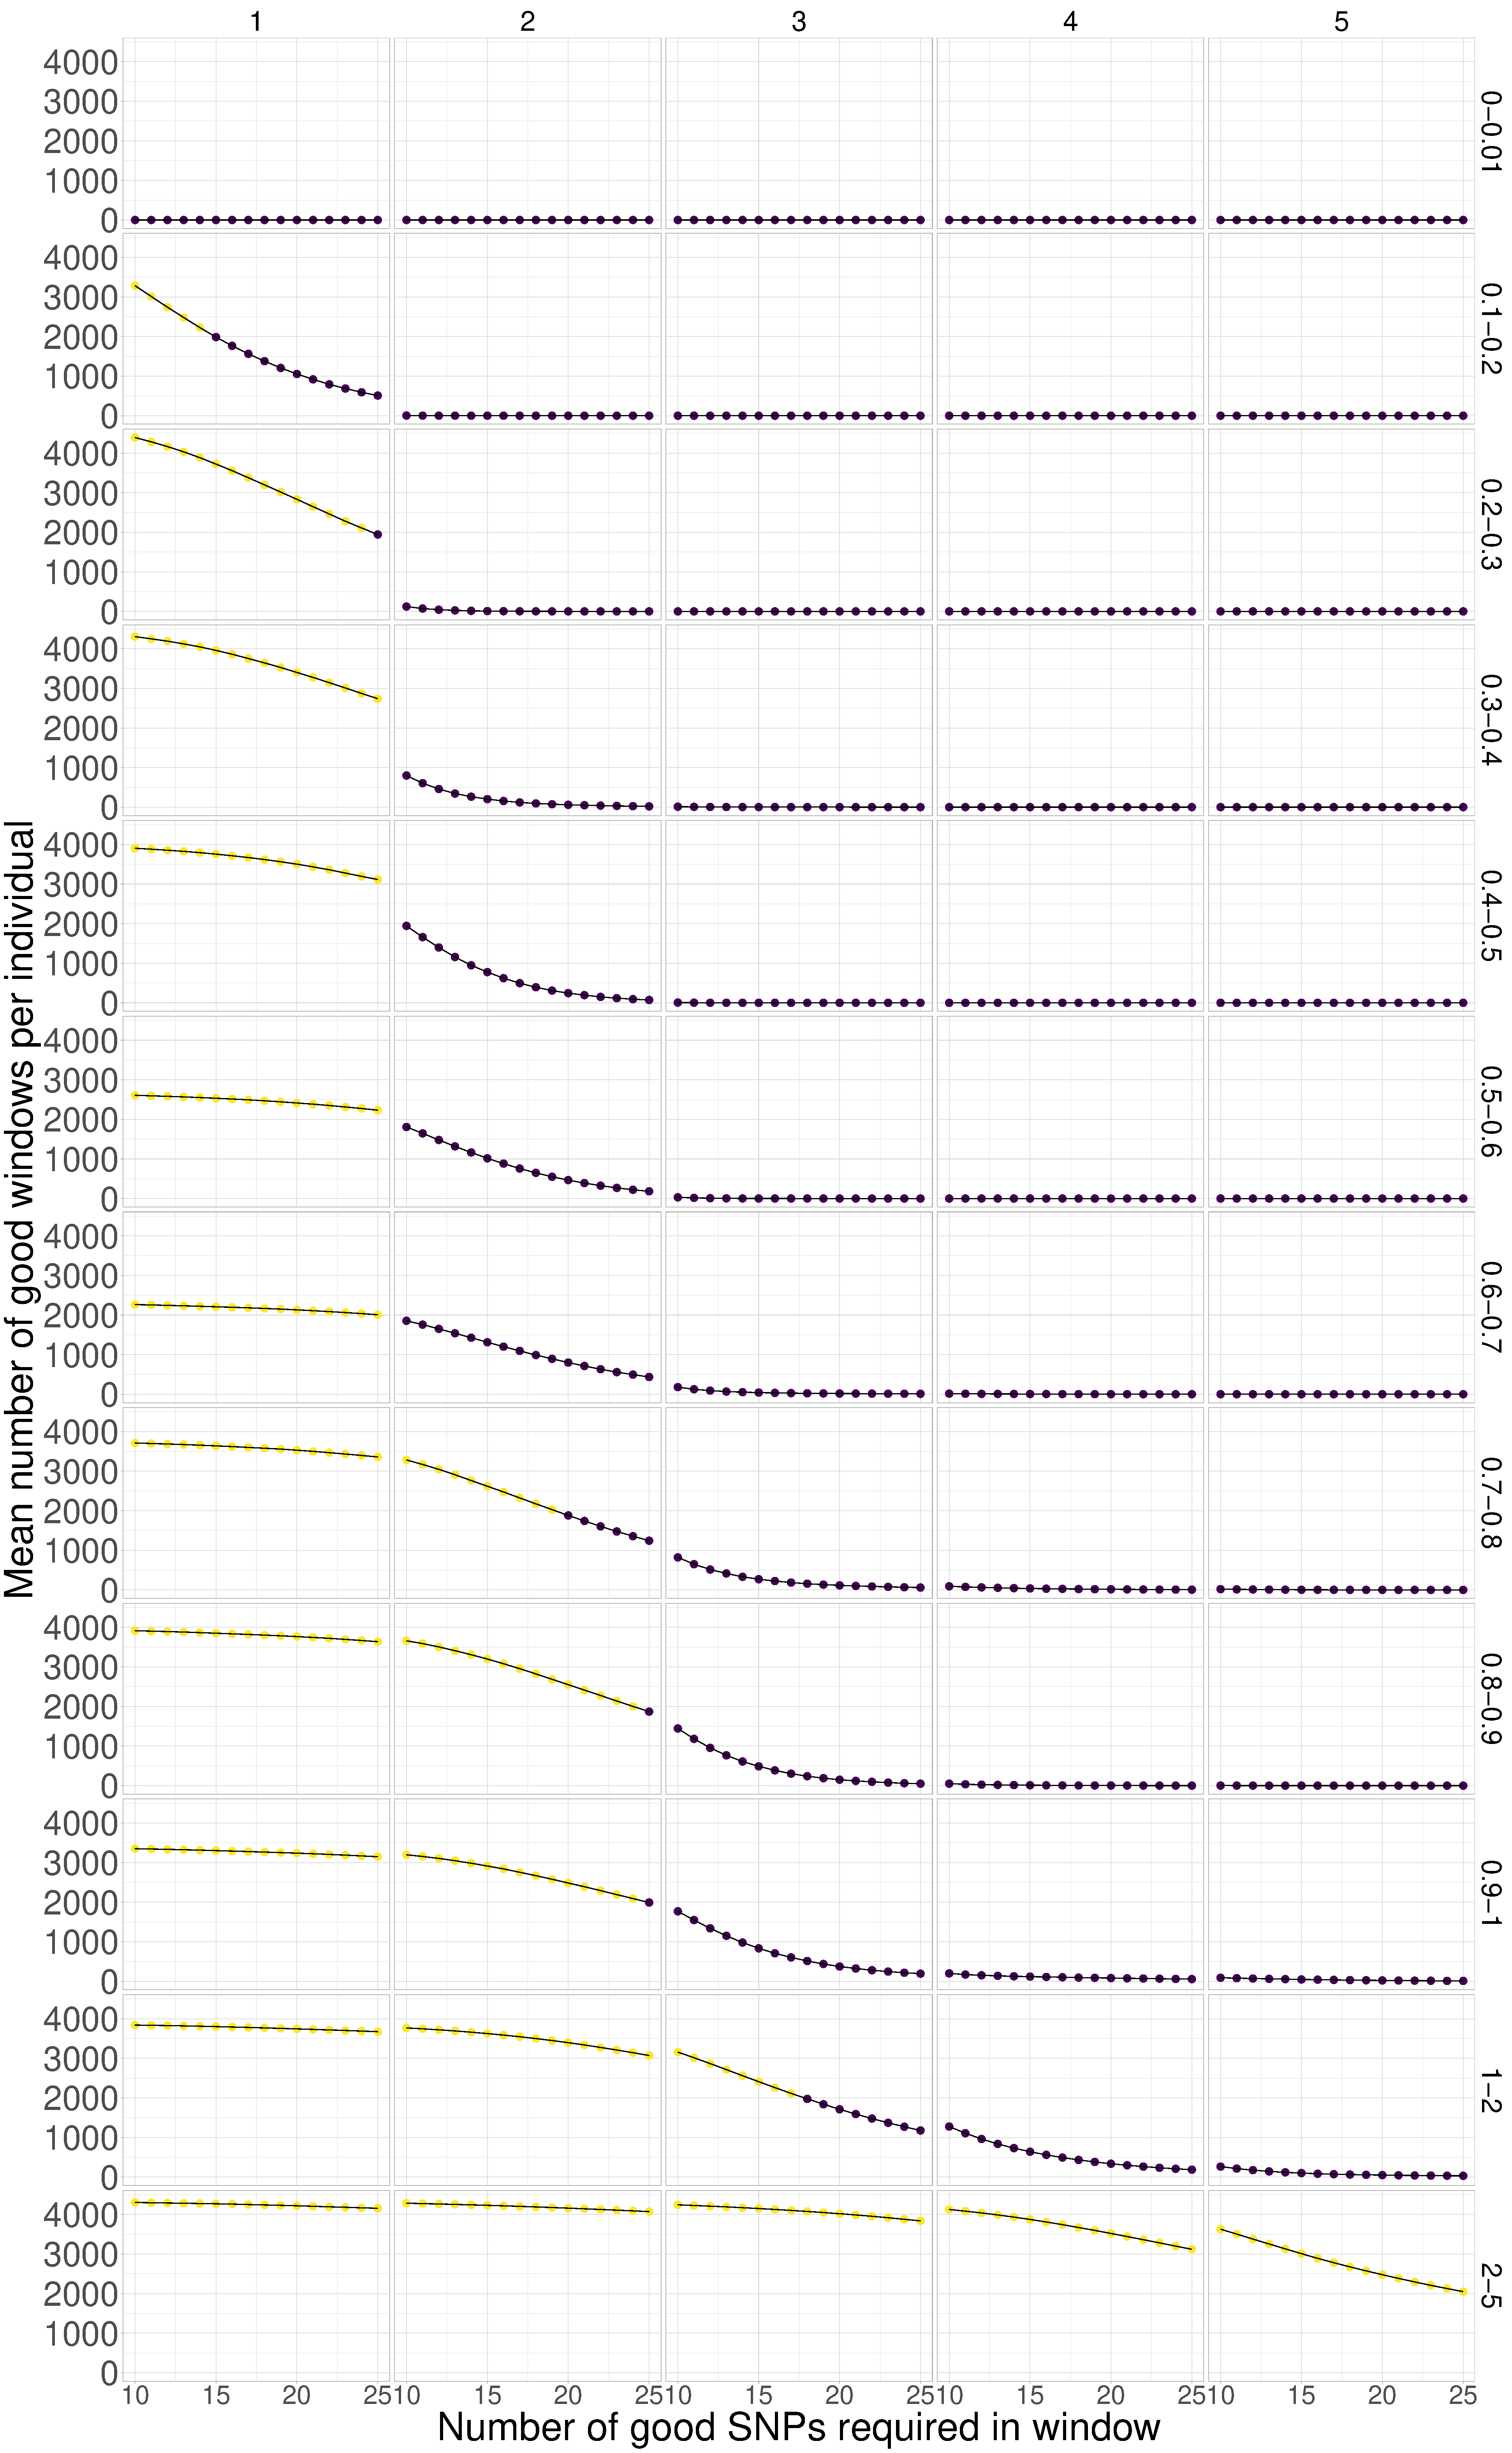
\includegraphics[width=1.0\textwidth]{../images/chapter1/avg_good_windows.pdf}
    \caption{Number of windows (y-axis) within the genome each ancient individuals within a given range of coverages (rows) with at least $Y$ SNPs (x-axis) above a particular coverage $Z$ (columns)}
    \label{fig:avg_good_windows}
\end{figure}





\section{Discussion}

We only had a single downsampled sample - this isn't necessarily realistic and I think we would gain a lot of power if we had e.g. 10 0.5x samples from a population. 

Using moderns to estimate imputation accuracy - why, and why might it give different results to using ancients. 
